\chapter{Model Description}
\label{ch:chapter4}
As mentioned in Chapter 1, I am using a \Gls{csg} model of the \Gls{msbr}
\cite{robertson_conceptual_1971} to verify my \OpenMC implementation in
\SaltProc.

I picked the \Gls{msbr} because\ldots 

The \Gls{msbr} design is the result of a design study of a single-fluid
\Gls{msr} following the success of the \Gls{msre}
\cite{haubenreich_experience_1970}\cite{rosenthal_molten-salt_1970}.
I will only describe the following reactor systems that are relevant to
my validation study\footnote{A complete description of the entire \Gls{msbr}
system can be found in Robertson, et al (1971)\cite{robertson_conceptual_1971}.
Interested readers should pay close attention to Table S.1, Section 3.1, and
Section 3.4 in Robertson et al. for further details and design considerations.}:
the fuel salt, the reactor core, and the salt reprocessing system.

\begin{figure}[htpb] 
    \centering
    \subfloat[][]{
        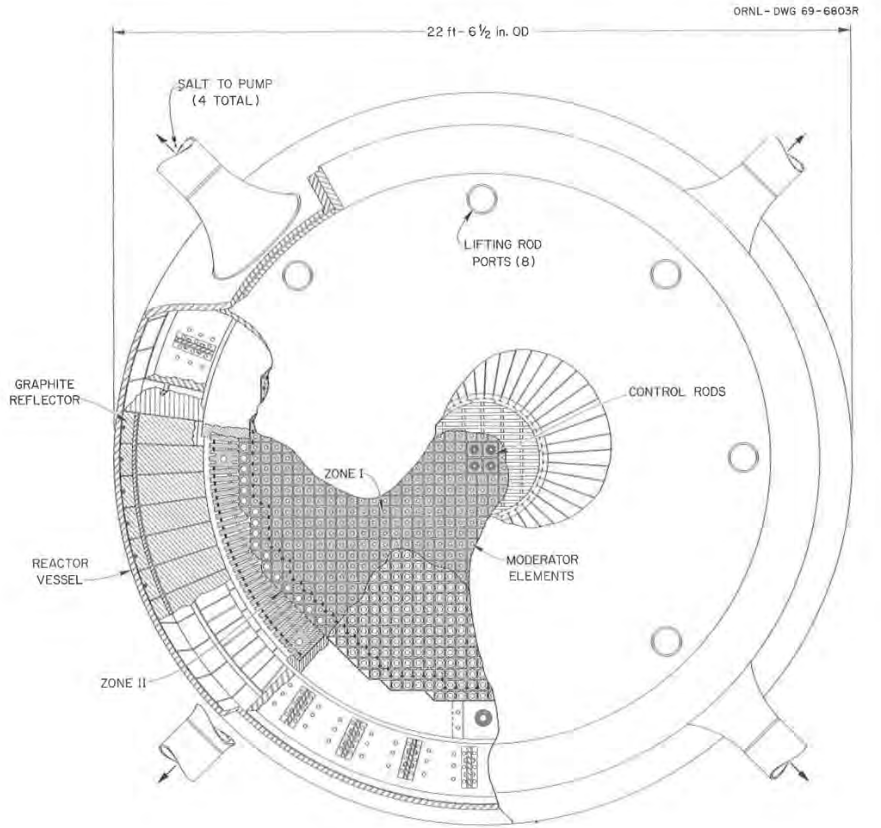
\includegraphics[width=0.5\linewidth]{figs/ch4/msbr_full_xy_ref.png}
        \label{fig:msbr-ref-xy}
    }
    \subfloat[][]{
        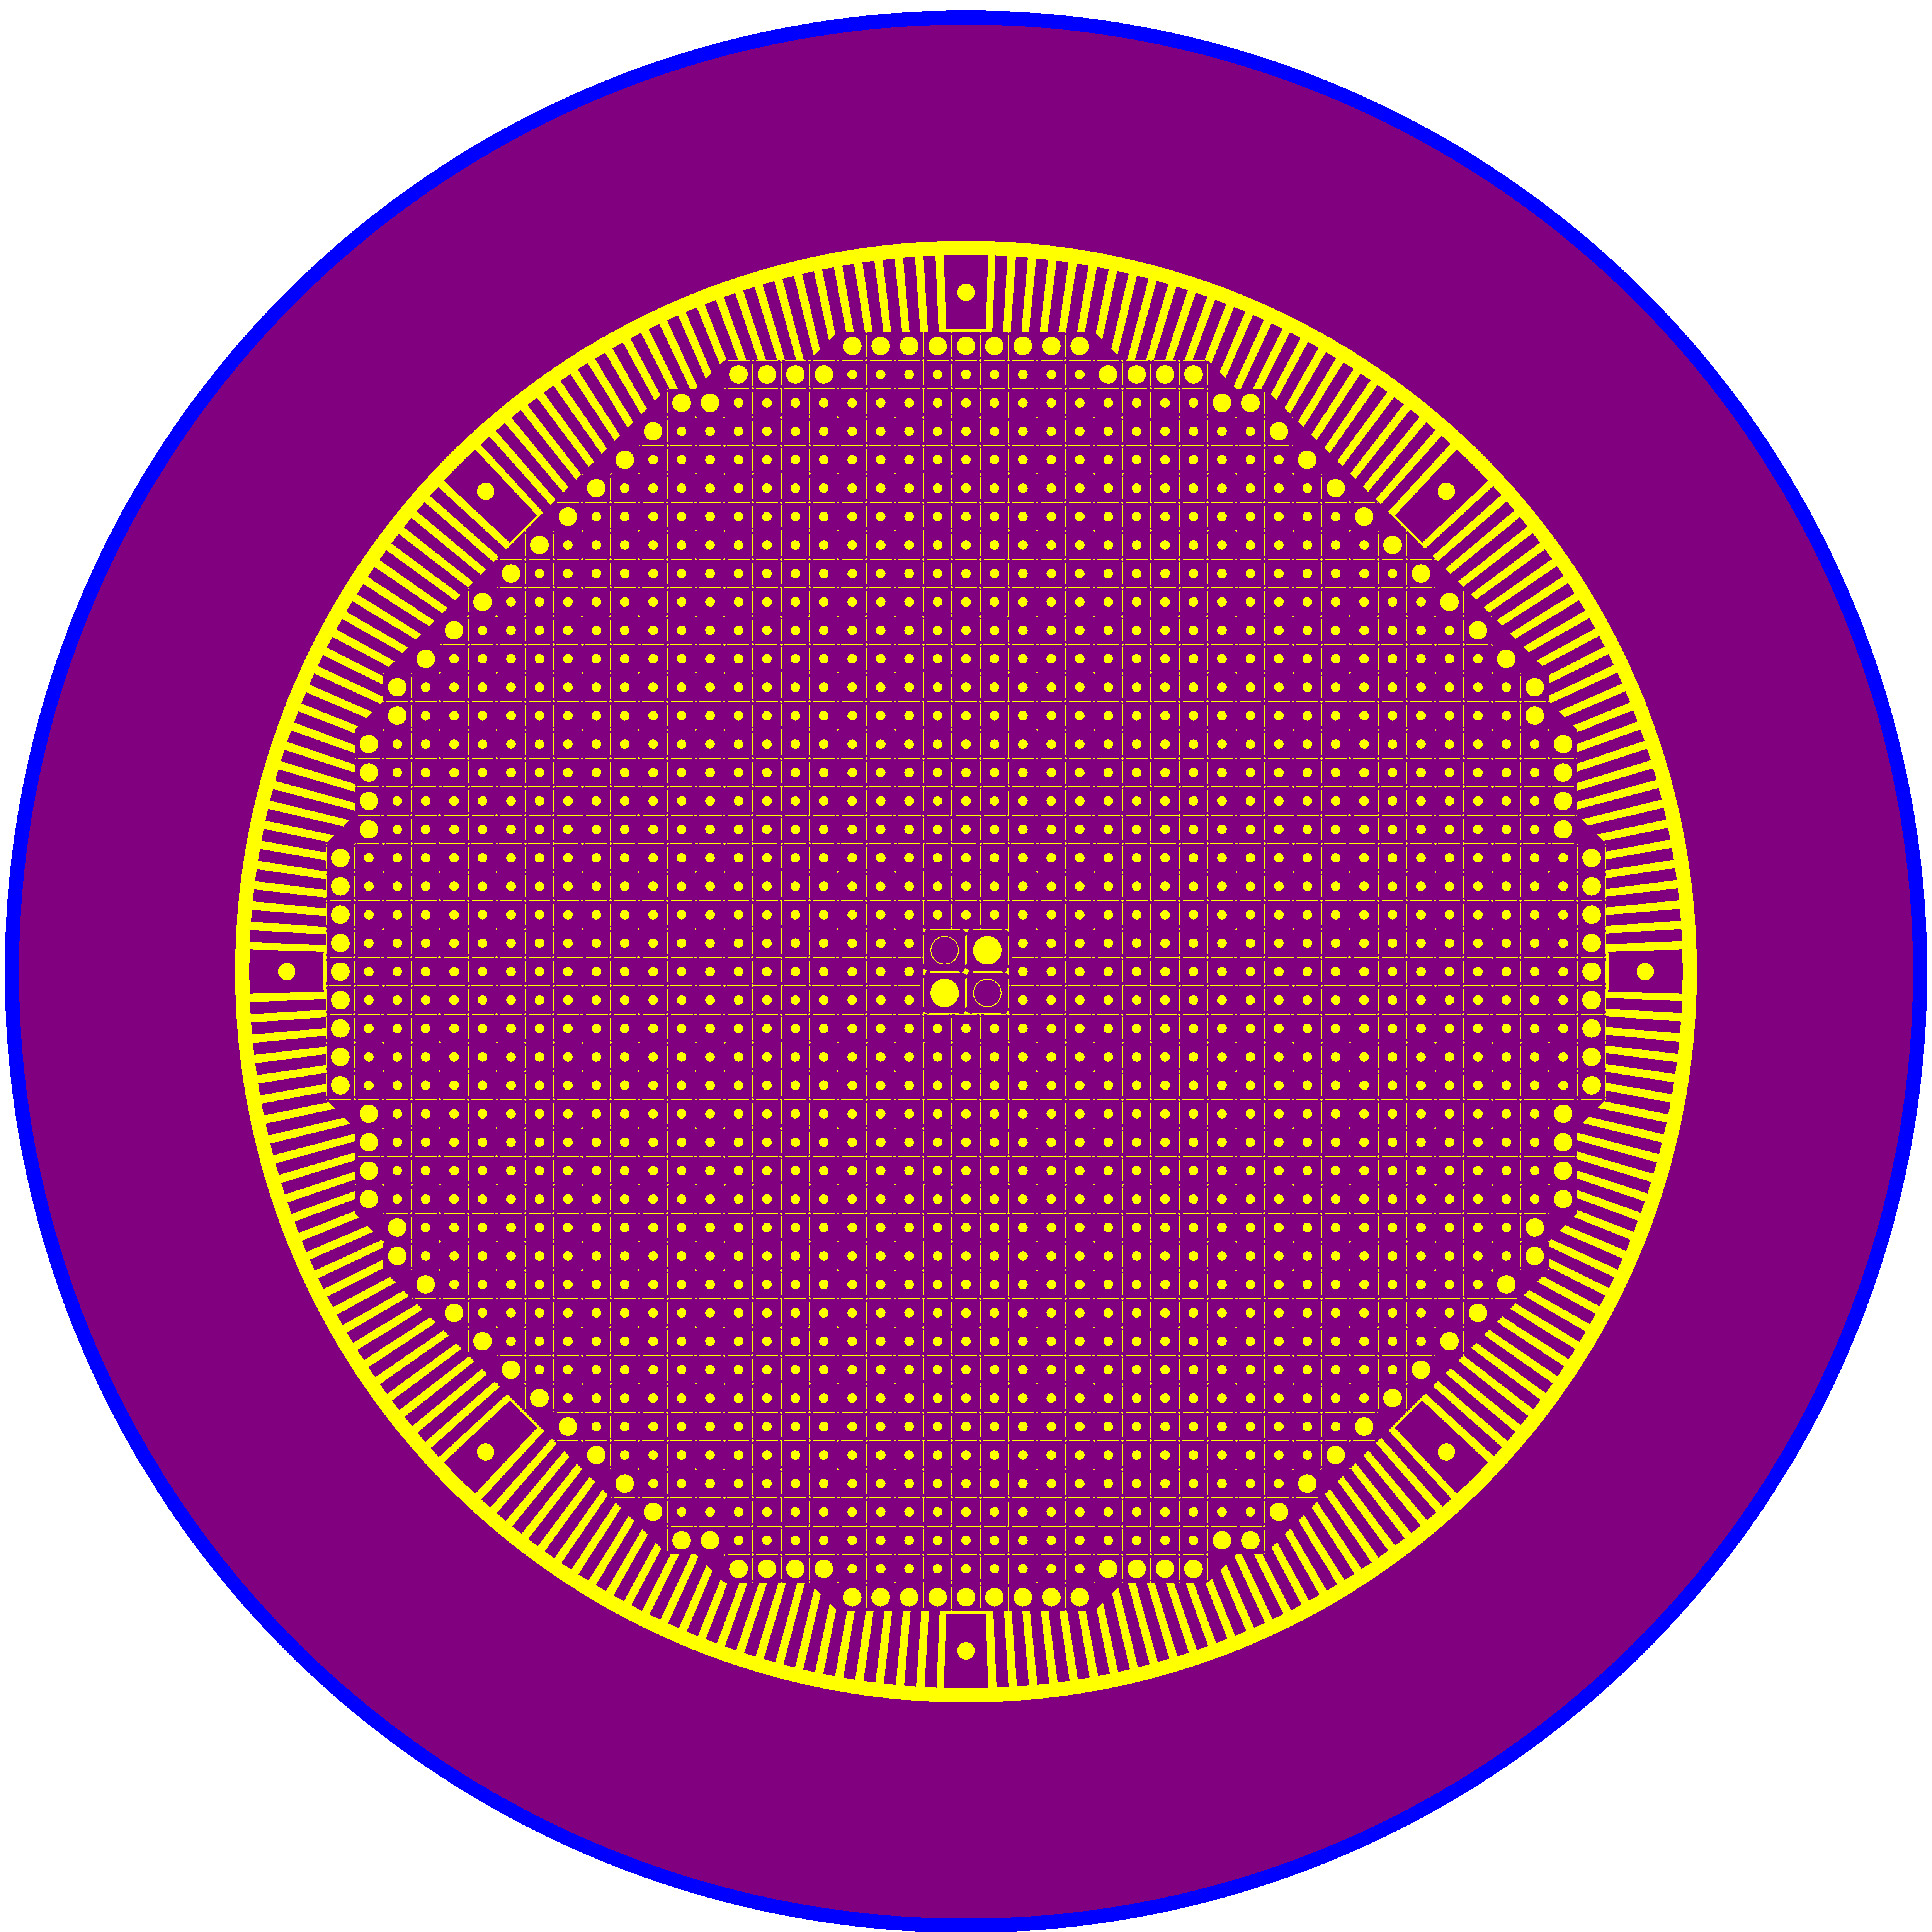
\includegraphics[width=0.5\linewidth]{figs/ch4/msbr_full_xy_openmc.png}
        \label{fig:msbr-model-xy}
    }
    \\
    \subfloat[][]{
        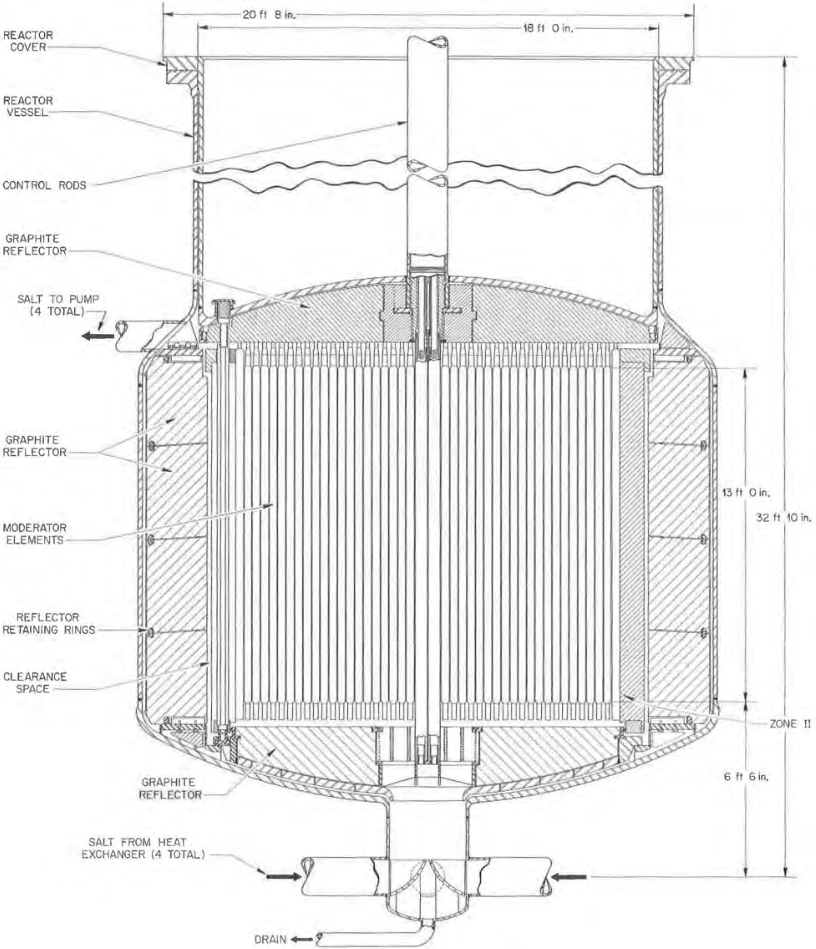
\includegraphics[width=0.5\linewidth]{figs/ch4/msbr_full_xz_ref.png}
        \label{fig:msbr-ref-xz}
    }
    \subfloat[][]{
        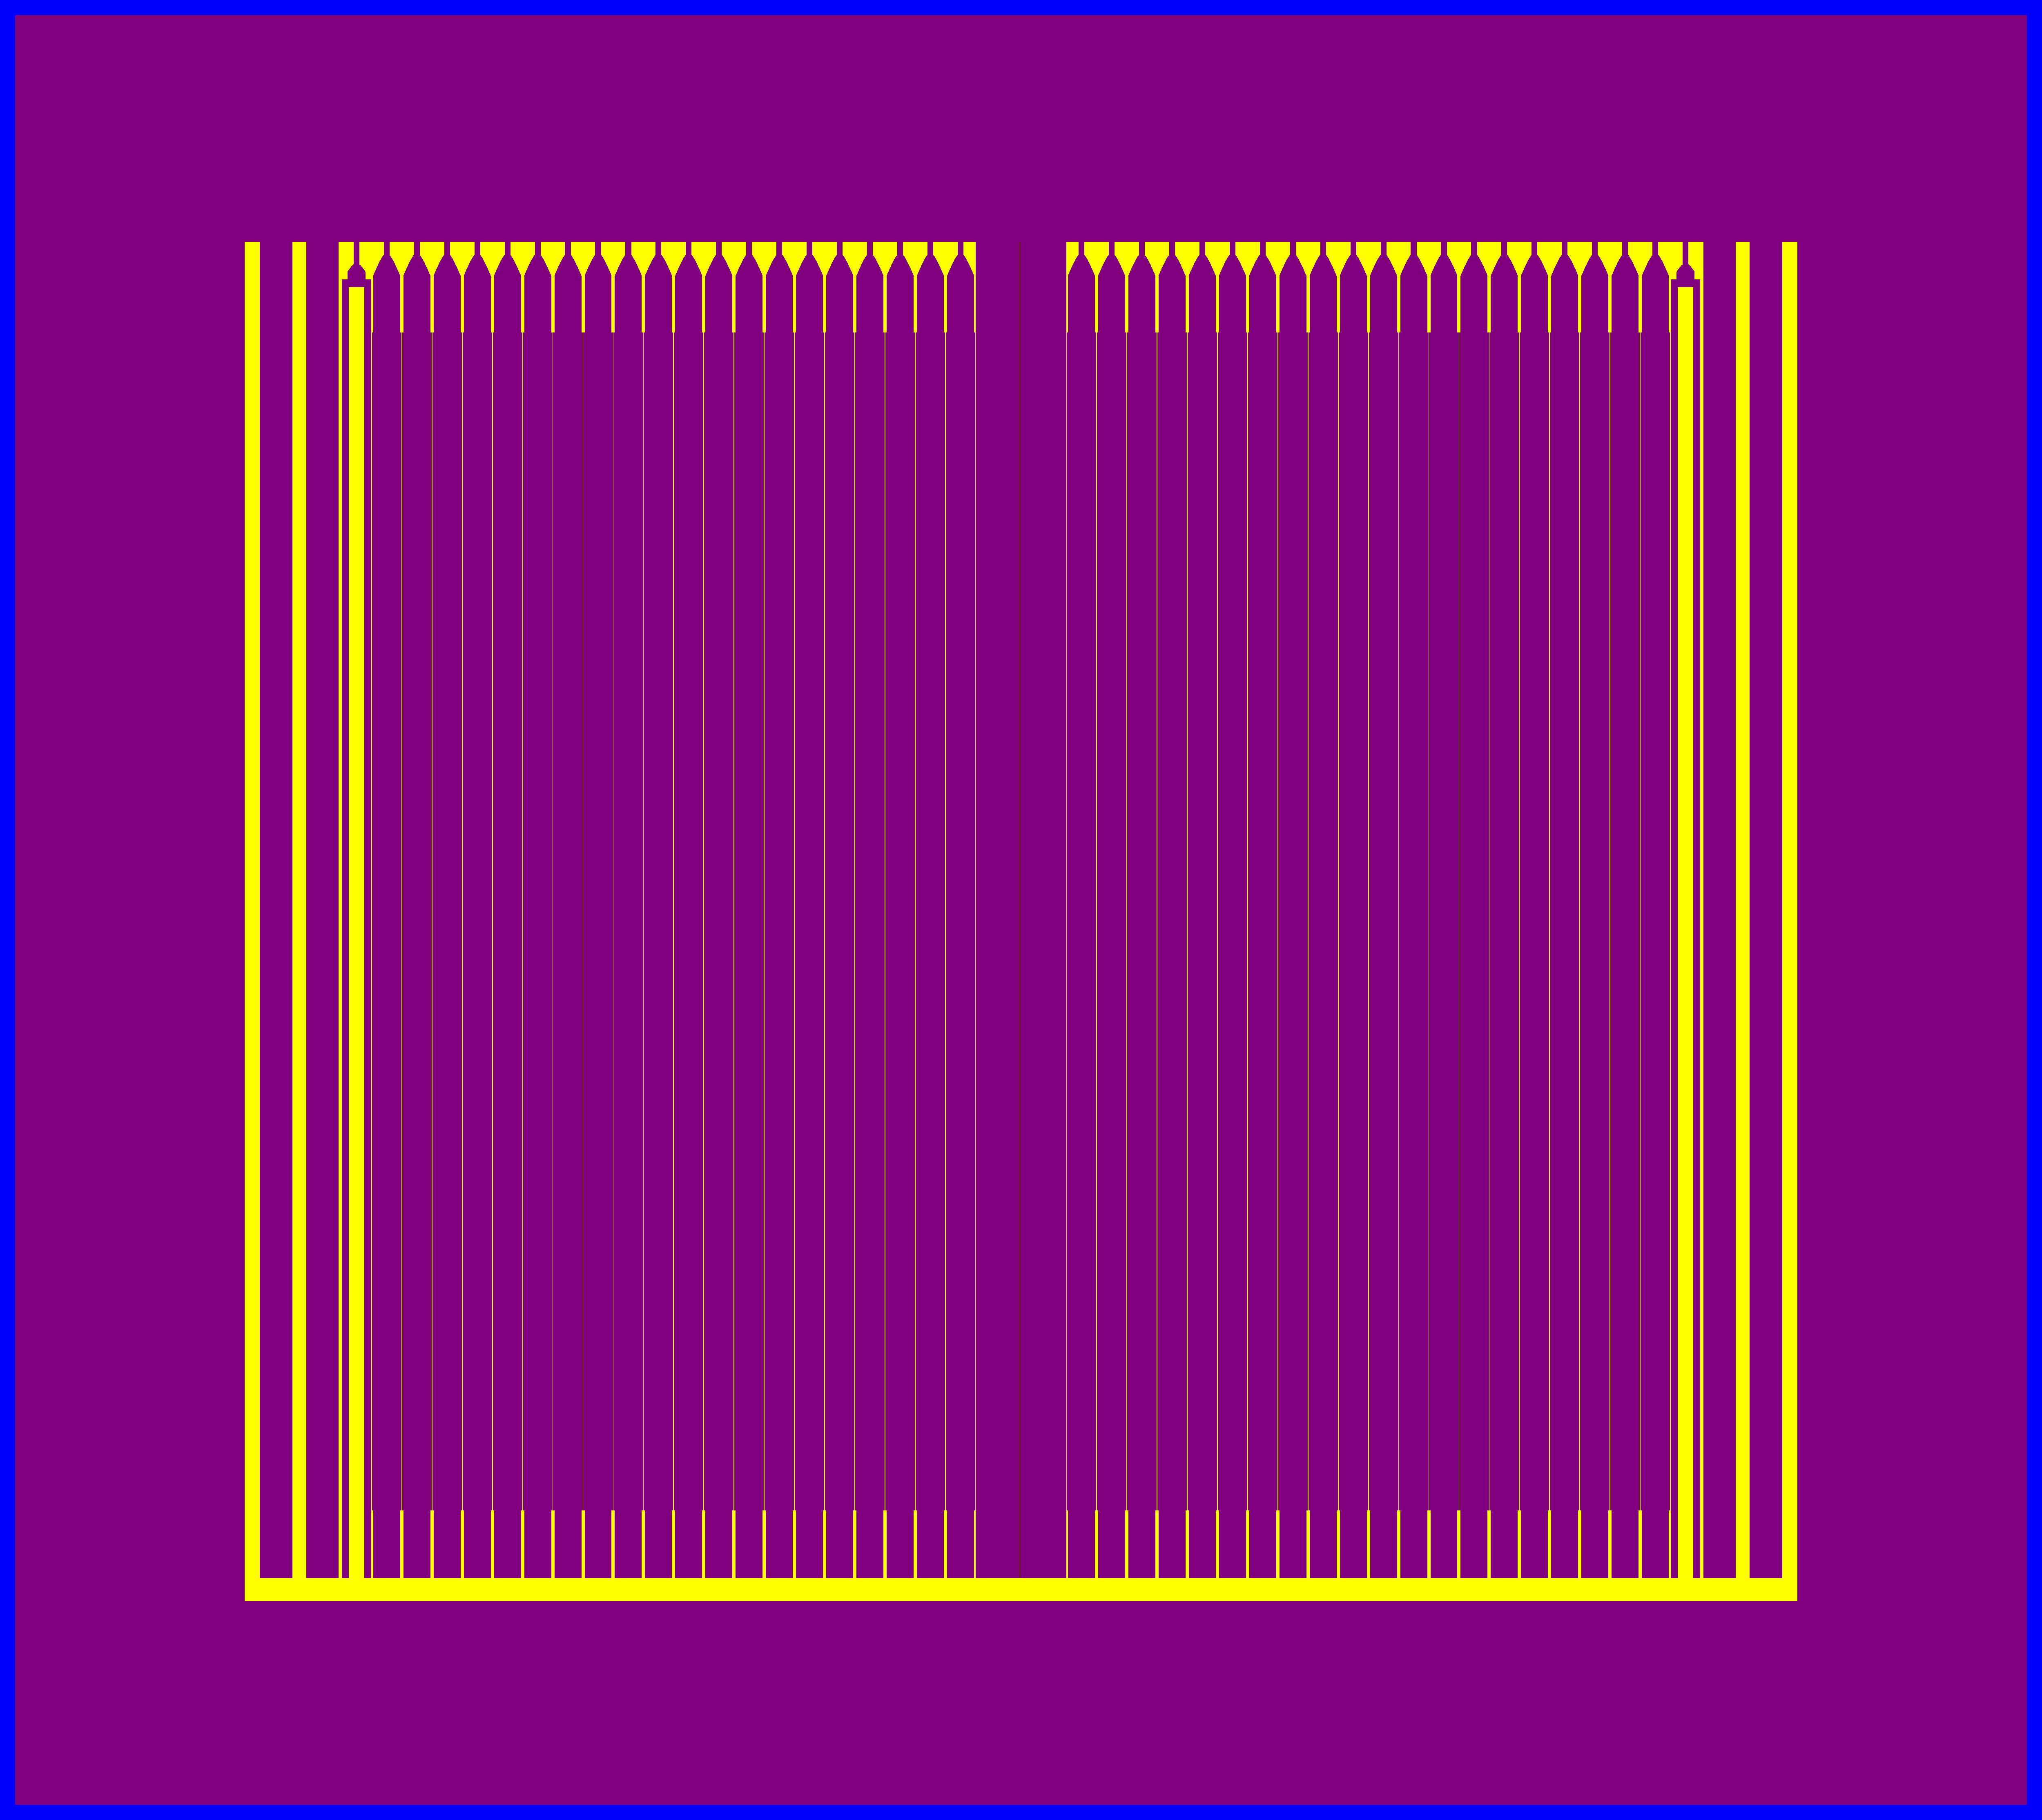
\includegraphics[width=0.5\linewidth]{figs/ch4/msbr_full_xz_openmc.png}
        \label{fig:msbr-model-xz}
    }
    \caption[Full views of MSBR]{
        \subref{fig:msbr-ref-xy} Top down view of \Gls{msbr} reference design.
        \subref{fig:msbr-model-xy} Top down view of \Gls{msbr} CSG model.
        \subref{fig:msbr-ref-xz} Side view of \Gls{msbr} reference design.
        \subref{fig:msbr-model-xz} Side view of \Gls{msbr} CSG model.
    }
    \label{fig:msbr-overview}
\end{figure}

As seen in Figure \ref{fig:msbr-overview} \OpenMC and \SerpentTWO \Gls{msbr}
models of reproduce these systems with several approixmations. I will
describe each reactor system, as well as any relavant changes or
approximations made in the model.

\section{Materials}
\label{sec:msbr-materials}

\subsection{Fuel salt}
\label{sub:msbr-fuel-salt}
Table S.1 in \cite{robertson_conceptual_1971} specifies the fuel salt
composition used in the \Gls{msbr}:
\ce{LiF}-\ce{Be}\ce{F_2}-\ce{Th}\ce{F_4}-\ce{U}\ce{F_4} at a
concentration of 71.7-16-12-0.3 mole-\%\footnote{In Rykhlevskii's thesis
\cite{rykhlevskii_fuel_2020}, he stated the mole-\% to be 71.75-16-12-0.25. I
have been unable to find this composition in Robertson et al.
\cite{robertson_conceptual_1971}}. The lithium used in the fuel salt is
enriched to 99.995\% \ce{^{7}Li}. This is because \ce{^{6}Li} is a strong
neutron absorber and produces tritium in the absorption reaction. The atom-\%
for each nuclide is given in Table \ref{tab:msbr-fuel-salt-ref}\footnote{Most of the
discussion of the fuel salt compositon in Robertson el al
\cite{robertson_conceptual_1971} specify elemental version of the nuclides in
Table \ref{tab:msbr-fuel-salt-ref}. I have specific specific nuclides for the
following reasons: (1) both \ce{F} and \ce{Be} have only one stable isotope, (2)
the fuel salt recieves initial fissile loading from \ce{^{233}U} or
\ce{^{235}U}, and (3) the fuel salt recieves its fertile loading from
\ce{^{232}Th}}.

The original salt volume in the \Gls{csg} \Gls{msbr} model was set to
$4.871\cdot 10^7$ \unit{\centi\metre\cubed}. This is roughly double the salt
volume in the reference specification (see Table \ref{tab:salt-volumes}). I
performed stochastic volume calculations on both the \SerpentTWO and \OpenMC
versions of the \Gls{csg} model, and found they both calculated volumes around
$2.6\cdot 10^7$ \unit{\centi\metre\cubed}. I have updated the salt volume to the
average of the two volumes (see Table \ref{tab:stoch-vol}). This new volume
gives a rougly 8\% error in the salt volume compared to the reference
specification.

\begin{table}[htpb]
    \centering
    \caption[MSBR fuel stochastic volume calculations]{MSBR fuel stochastic volume calculations, using $1\cdot 10^9$ particles.}
    \label{tab:stoch-vol}
    \begin{tabular}{|c|c|c|c|}
        \hline
        Quantity & \SerpentTWO & \OpenMC & Average\\
        \hline
        Volume [\unit{\centi\metre\cubed}] & $2.60961 \cdot 10^7$ & $2.6085 \cdot 10^7$ & $2.6091 \cdot 10^7$ \\
        \hline
        Statistical error & 0.00010 & 0.00010 & 0.00007 \\
        \hline
    \end{tabular}
\end{table}

\begin{table}[htpb] 
    \centering 
    \caption{Reference \Gls{msbr} fuel salt specifications}
    \label{tab:msbr-fuel-salt-ref}
    \begin{tabular}{|c|c|c|c|c|c|c|} 
        \hline
        & \ce{^{6}Li} & \ce{^{7}Li} & \ce{^{19}F} & \ce{^{9}Be} & \ce{^{232}Th} & \ce{^{233}U}\\
        \hline 
        atom-\% & 1.4357925 & 34.4142075 & 56.35$\overline{6}$ & 5.$\overline{3}$ & 2.4 & 0.06 \\
        \hline
        mass-\% & 0.4452449 & 12.4477343 & 55.1982285 & 2.4779439 & 28.7100003 & 0.7208481\\ 
        \hline
    \end{tabular}
\end{table}

The density of the fuel salt is given by a function\footnote{This function 
comes from an earlier report on the Molten-Salt Reactor Program
\cite{rosenthal_molten-salt-ornl_1970}.} of temperature in \unit{\celsius} in Table
S.1 in Robertson et al. \cite{robertson_conceptual_1971}:
\begin{equation}
    \rho = 3.752 - 6.68\cdot 10^{-4} \cdot T \quad \unit{\gram\per\square  \centi\meter}
\end{equation}

The temperature of the fuel salt flowing into the core at the inlet at the
bottom of the reactor is 1050\unit{\degree}F (565.5556\unit{\celsius}, 838.7056
\unit{\kelvin}), and the temperature of the fuel salt flowing out of the core at
the outlet is approximately 1300\unit{\degree}F (704.4444\unit{\celsius},
977.5944 \unit{\kelvin})\cite{robertson_conceptual_1971}. The average
temperature of the salt over the core inlets and outlets is then 1175
\unit{\degree}F (635\unit{\celsius}, 908.15 \unit{\kelvin}). While the
various solid components of the core are at a slightly higer temperature on
average\footnote{see figure 3.29 in \cite{robertson_conceptual_1971}}, for
simplicity, I set the evaluated temperature of all materials to 900
\unit{\kelvin} consistent cross-section selection between the \OpenMC and
\SerpentTWO depletion steps. At this temperature, the density of the fuel salt
is 3.3332642 \unit{\gram\per\centi\metre\cubed}.

\begin{table}[htpb] 
    \centering 
    \caption{Model \Gls{msbr} fuel salt specifications}
    \label{tab:msbr-fuel-salt-model}
    \begin{tabular}{|c|c|c|c|c|c|} 
        \hline
        & \ce{^{7}Li} & \ce{^{19}F} & \ce{^{9}Be} & \ce{^{232}Th} & \ce{^{233}U}\\
        \hline 
        atom-\% & 28.386326 & 60.437153 & 6.330058 & 4.747557 & 0.098907 \\
        \hline
        mass-\% & 7.87474673879085 & 45.4003012179284 & 2.25566879138321 & 43.5579130482336 & 0.911370203663893\\ 
        \hline
    \end{tabular}
\end{table}
In the CSG model, the fuel salt material uses the composition specified in
Table \ref{tab:msbr-fuel-salt-model} and has a density of 3.35
\unit{\gram\per\centi\metre\cubed}. Notice that the lithium has been enriched to
100\% \ce{^{7}Li}. This is because during inital simulations, even those very
small amounts of \ce{^{6}Li} were enough to kill the reaction. The inital
fissile and fertile loading has also been slightly increased.

\subsection{Graphite}
\label{sub:graphite}

For a detailed description of the reactor graphite used in the \Gls{msbr}, see
Section 3.2.3 in \cite{robertson_conceptual_1971}. At 70\unit{\degree}F (294.3
\unit{\kelvin}), the \Gls{msbr} graphite has a density of 1843
\unit{\kilo\gram\per\cubic\metre}. This is the only density specification
for graphite that I was able to find in Robertson et al.
\cite{robertson_conceptual_1971}

In the CSG model, the graphite material uses elemental carbon and has a
density of 1.84\unit{\gram\per\centi\metre\cubed}.

\subsection{Modified Hastelloy N}
\label{sub:hastelloy}
Hastelloy N is an alloy developed at \Gls{ornl} during the Molten-Salt Reactor
Program as a structural material that could maintain structural stability while
in contact with the corrosive and high temperature molten salt fuel while also
being under irradation for a long period of time.

The \Gls{msbr} used a modified version of Hastelloy N designed to improve
embrittlement resistance and weldibility \cite{robertson_conceptual_1971}.
The \Gls{msbr} uses modified Hastelloy N on all nearly all salt-facing
components included in the CSG model.

Modified Hastelloy N has a density of 8671 \unit{\kilo\gram\per\cubic\metre} at
1300\unit{\degree}F (704.4444\unit{\celsius}, 977.5944 \unit{\kelvin})
\cite{robertson_conceptual_1971}. The elemental composition of modified
Hastelloy N and their amounts in mass-\% are in Table \ref{tab:hastelloy-n-ref}.

\begin{table}[htpb]
    \centering
    \caption[Mass-\% of elements in modified Hastelloy N used in the \Gls{msbr}]{Mass-\% of elements in modified Hastelloy N used in the \Gls{msbr}. Data from Table 3.1 and S.1 in \cite{robertson_conceptual_1971}. Ranged values collapsed to their average are denoted with a $^*$}
    \label{tab:hastelloy-n-ref}
    \begin{tabular}{|c|c|c|c|c|c|c|c|c|c|c|c|c|c|c|c|c|}
        \hline
        \ce{Ni} & \ce{Mo}$^*$ & \ce{Cr}$^*$ & \ce{Fe}$^*$ & \ce{C}$^*$ & \ce{Mn}$^*$ & \ce{Si} & \ce{W} & \ce{Al} & \ce{Ti}$^*$ & \ce{Cu} & \ce{Co} & \ce{P} & \ce{S} & \ce{B} & \ce{Hf}$^*$ & \ce{Nb}$^*$ \\
        \hline
        73.709 & 12 & 7 & 3 & 0.06 & 0.35 & 0.1 & 0.1 & 0.1 & 1.25 & 0.1 & 0.2 & 0.015 & 0.015 & 0.001 & 1 & 1\\
        %\hline
        %atom-\% & 76.72 & 7.64 & 8.224 & 3.282 & 0.305 & 0.389 & 0.218 & 0.033 & 0.226 & 1.595 & 0.096 & 0.207 & 0.03 & 0.029 & 0.006 & 0.342 & 0.658 \\
        \hline
    \end{tabular}
\end{table}

\begin{table}[htpb]
    \centering
    \caption{Mass-\% of elements in modified Hastelloy N used in the \Gls{msbr} model.}
    \label{tab:hastelloy-n-model}
    \begin{tabular}{|c|c|c|c|}
        \hline
        \ce{Ni} & \ce{Cr} & \ce{W} & \ce{Al} \\
        \hline
        67.7 & 7.0 & 25.0 & 0.3 \\
        \hline
    \end{tabular}
\end{table}

The Hastelloy N material in the CSG model uses the composition specified in
Table \ref{tab:hastelloy-n-model} and has a density of 8.671 
\unit{\gram\per\centi\metre\cubed}. The model material has a different composition
than the reference material because\ldots


\section{Reactor core}
\label{sec:msbr-core}
The \Gls{msbr} core is split into three distinct different zones; zone I, zone
II, and the reflector zone. 

%% Table 3.2 and 3.3 in robertson
\begin{table}[htpb]
    \centering
    \caption[Volume of salt in reference MSBR core regions]{Volume of salt in
reference MSBR core regions. Reproduced from Table 3.2 in
\cite{robertson_conceptual_1971}}
    \label{tab:salt-volumes}
    \begin{tabular}{|c|c|cc|}
        \hline
        Zone & Percent salt & Salt volume [ft$^3$] & Salt volume [$10^6$\unit{\centi\metre\cubed}] \\
        \hline
        Zone I & 13.2 & 288 & 8.155252 \\
        \hline
        Zone II & 37 & 376.5 & 10.661293 \\
        \hline
        Upper plenum & 85 & 36.2 & 1.02507 \\ 
        \hline
        Lower plenum & 100 & 35.4 & 1.002416 \\ 
        \hline
        Annulus & 100 &  132 & 3.737824\\
        \hline
        Core total & - & 868.1 & 24.581855 \\ 
        \hline
    \end{tabular}
\end{table}

\begin{figure}[htpb]
    \centering
    \subfloat[][]{
        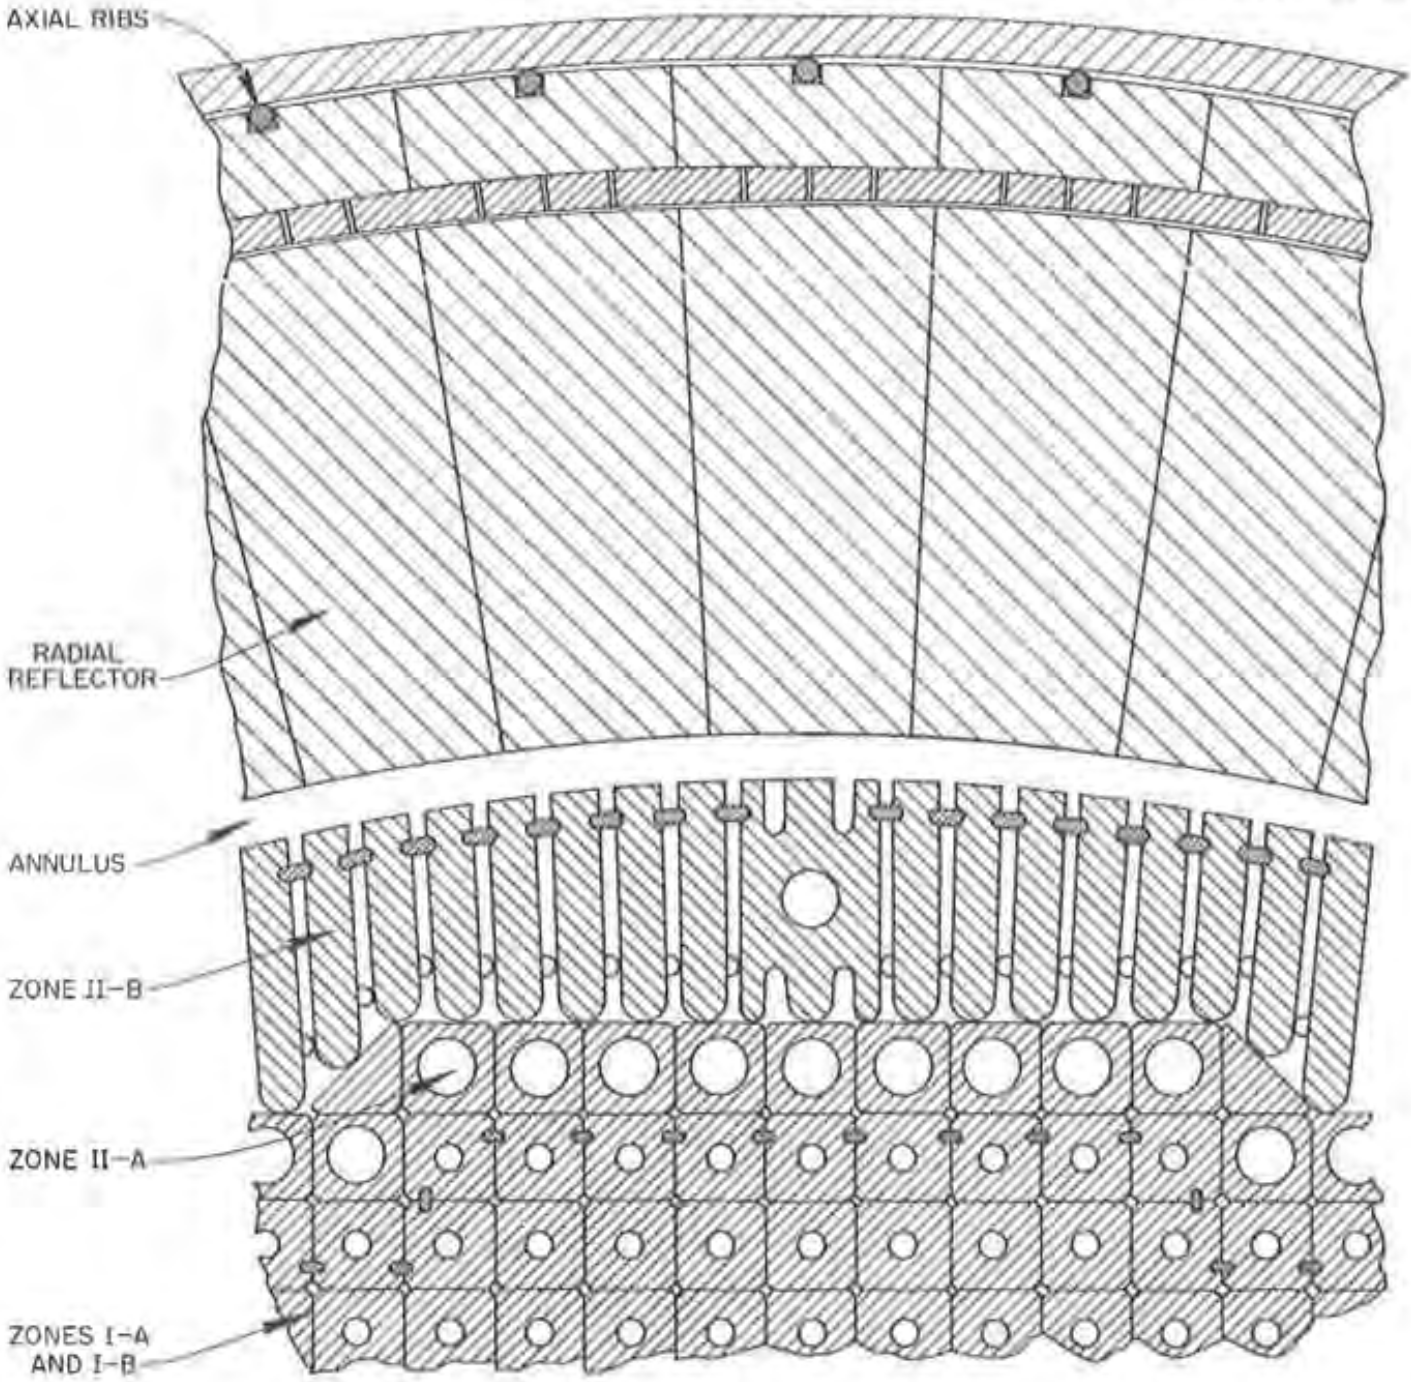
\includegraphics[width=0.45\linewidth]{figs/ch4/msbr_section_ref.png}
        \label{fig:msbr_sec_ref}
    }
    \subfloat[][]{
        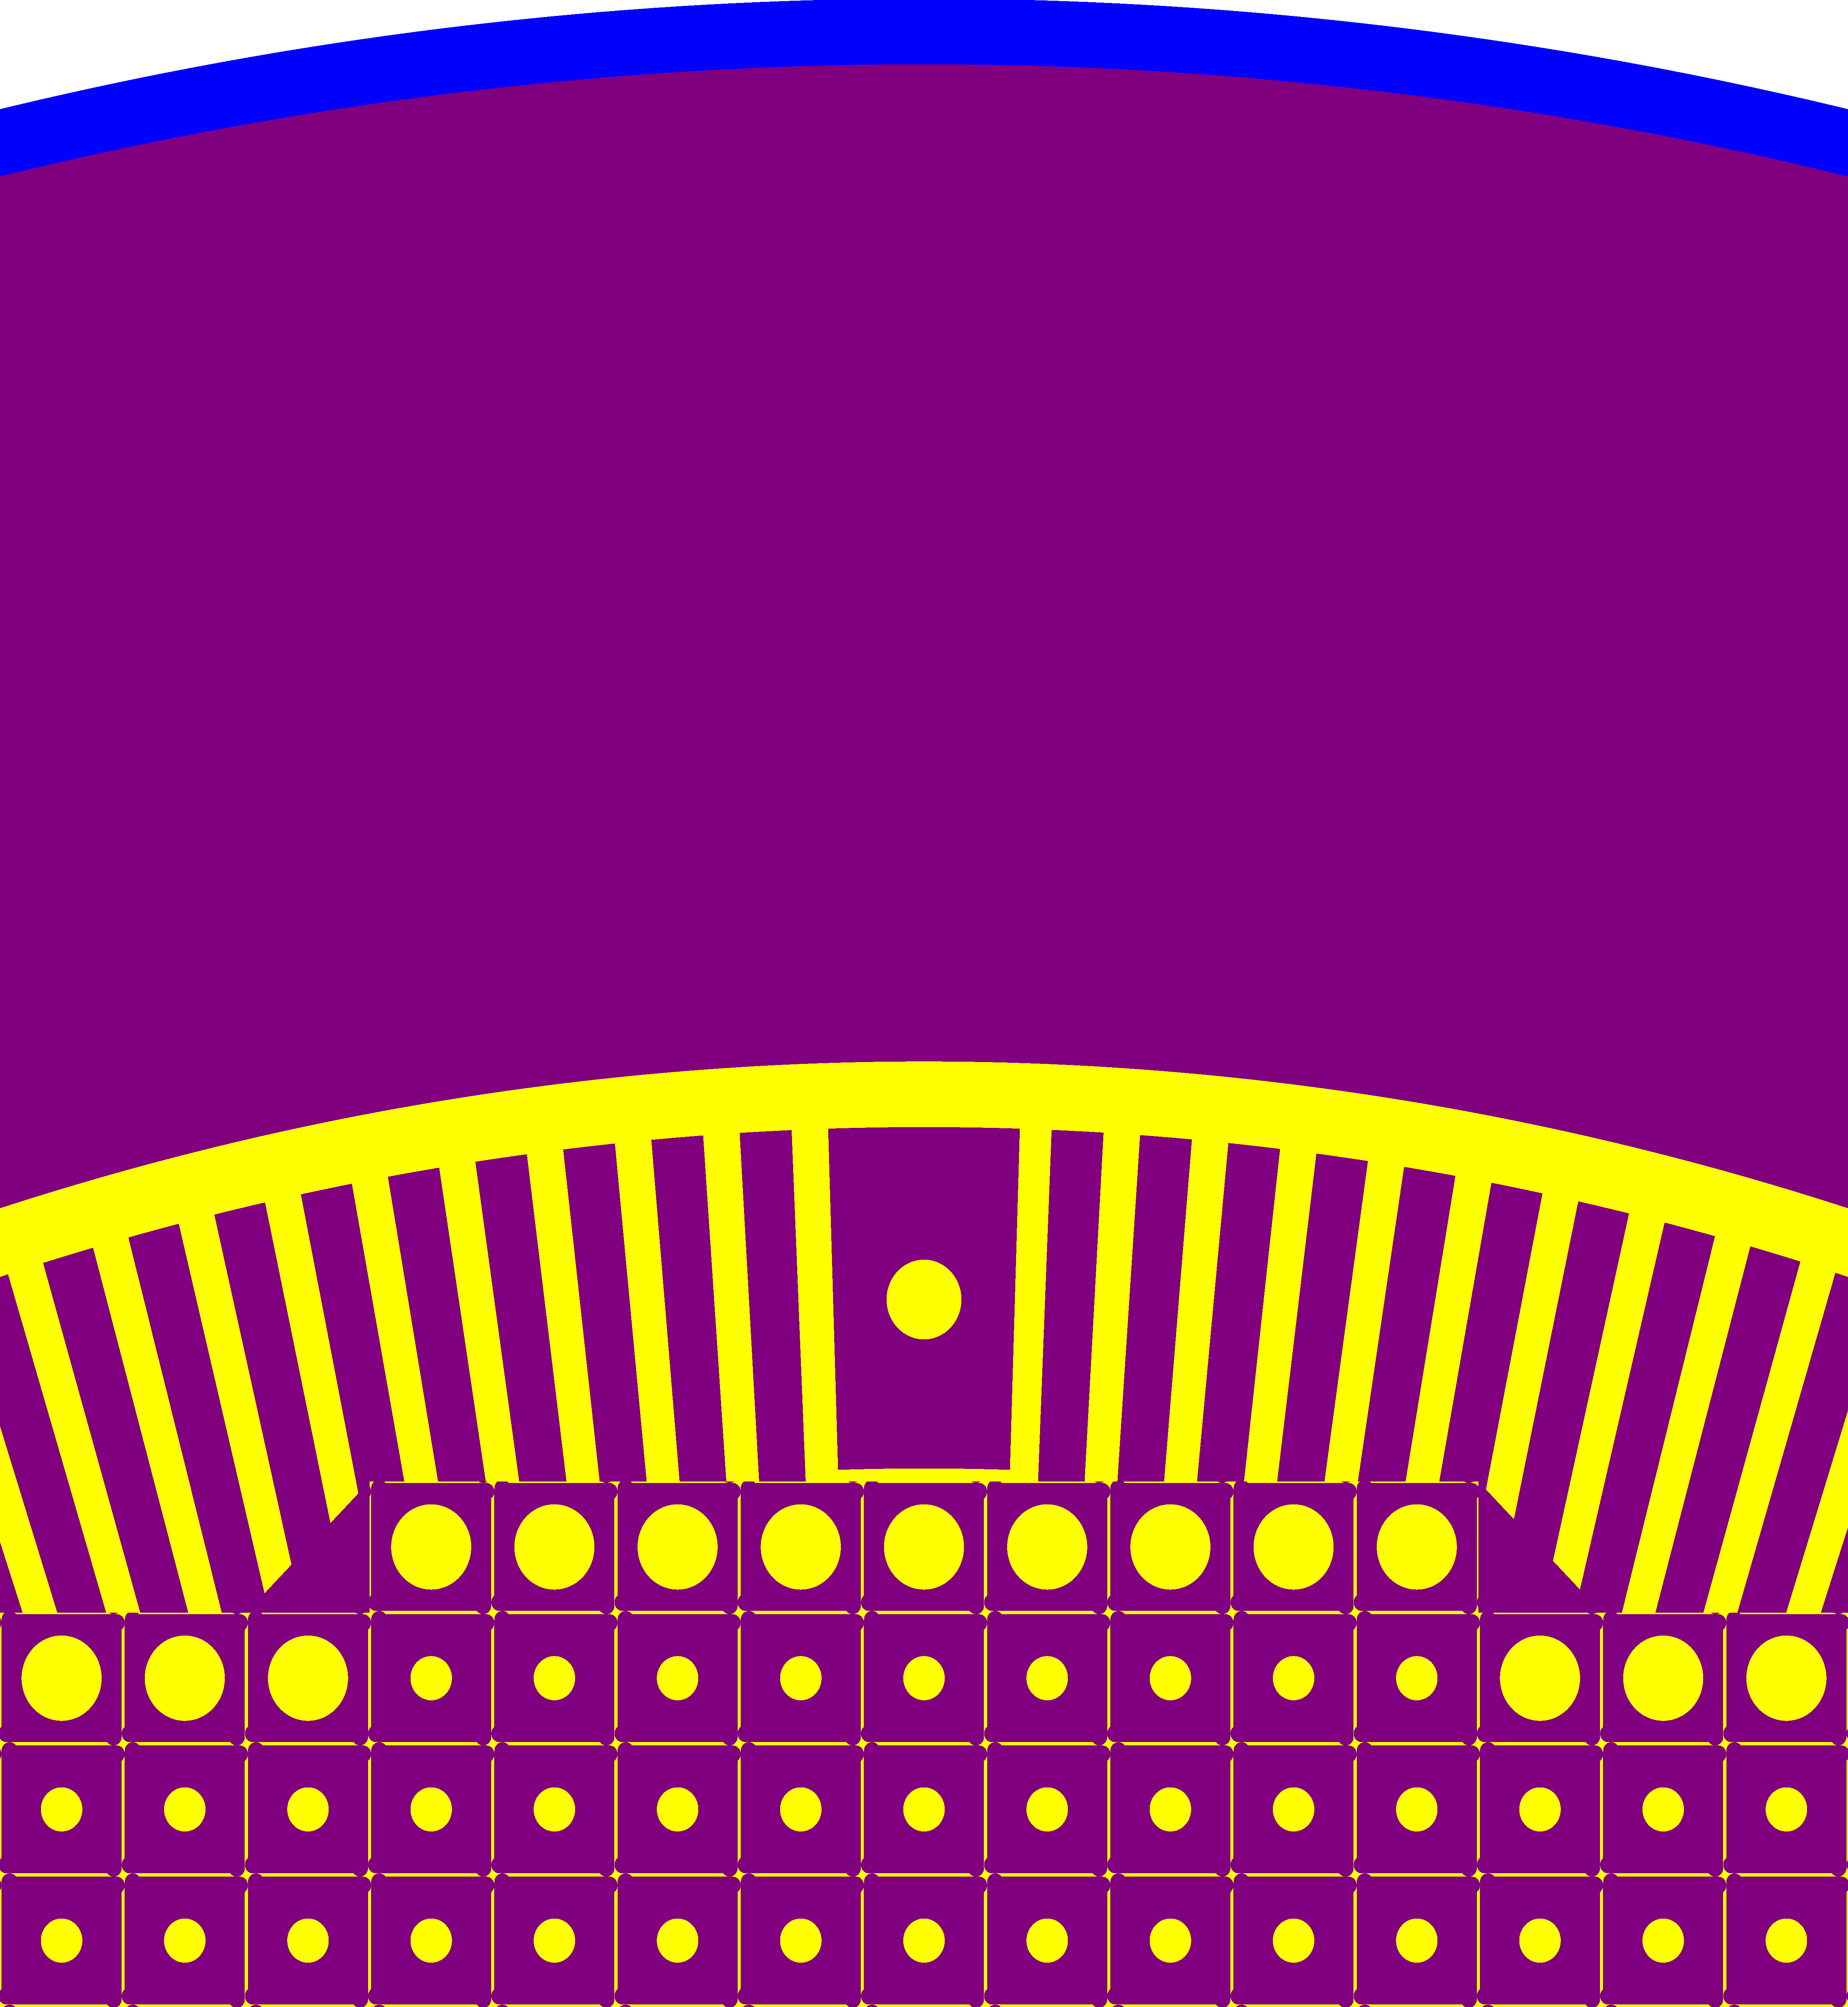
\includegraphics[width=0.35\linewidth]{figs/ch4/msbr_section_openmc.png}
        \label{fig:msbr_sec_model}
    }
    \caption[Detail views of MSBR core region]{
        \subref{fig:msbr_sec_ref} Detail view of \Gls{msbr} reference design.
        \subref{fig:msbr_sec_model} Detail view of \Gls{msbr} CSG model.}

    \label{fig:msbr-detail}
\end{figure}

\subsection{Zone I} Zone I is the central-most region of the core, and is 13.2\%
fuel salt by volume. Zone I is divided into three subzones: zone I-A, zone I-B,
and the control rod zone.

Zone I-A and I-B consist of 4-in.$\times$4-in. (10.16-cm$\times$10.16-cm)
square graphite elements. As seen in Figures \ref{fig:msbr-ia-xy} and
\ref{fig:msbr-ib-xy} elements in both zones have axial ribs protruding from
the faces of the square elements near the corners, as well as cylindrical
channels in the centers of the elements. The purpose of the fuel holes are to
facilitate salt flow through the core elements. The purpose of the ribs are to
separate the elements from each other as well as create interstitial salt flow
channels\cite{robertson_conceptual_1971}. These interstitial flow channels
are seen in Figures \ref{fig:msbr-ia-lattice} and
\ref{fig:msbr-ib-lattice}\footnote{Notice that the shape of the model zone I-B
elements qualitatively matches the reference design in Figure
\ref{fig:msbr-ib-xy}, but  not in Figure \ref{fig:msbr-ib-lattice}, despite
matching nearly all specifications of the reference design.}.

The only dimensional differences between the zone I-A and I-B elements are the
diameter of the cylindrical fuel channels and the size of the axial ribs (see
Tables \ref{tab:zone-ia-ref-specs} and \ref{tab:zone-ib-specs}). Zone I-A
elements have a smaller cylindrical channel and larger interstitial channel
than zone I-B elements. The central part of zone I consists of zone I-A
elements, whereas the outer part of zone I consists of zone I-B
elements\cite{robertson_conceptual_1971}. The purpose this configuration is to
reduce the temperature gradient across the core. The salt velocity through the
zone I-B elemets is much lower than the salt velocity through the zone I-A
elements\footnote{Robetson et al states that the salt velociy varies ``from 8
fps at the cetner [of the core] to about 2 fps near the
perihpery''\cite{robertson_conceptual_1971}}.

Additionally the zone I elements are machined to a cylindrical shape at the ends
to create an undermoderated region of 37\% salt at the top and bottom of the
reactor\cite{robertson_conceptual_1971}. These machined ends are referred to as
Section A (see Figures \ref{fig:msbr-ia-xy}, \ref{fig:msbr-ib-xy}, and
\ref{fig:msbr-i-xz-full}). The top of each element also has an outlet plenum to
direct salt flow towards the exit nozzlese at the edje of the vessel, however
these are not included in the \Gls{csg} model. The outermost layer of zone I
elements also have grooves in them to fit eliptical graphite sealing rods (see
Figure \cite{fig:msbr-detail}) that separate the salt flow in zone I from the
salt flow in zone II\cite{robertson_conceptual_1971}. Robertson et al does not
specify precise dimensions and positions of these rods, so they are not included
in the \Gls{csg} model.

Robertson et al. does not specify exact distribution of zone I-A and I-B
elements. Rather than guess the distribution of I-A and I-B elements, the CSG
model assumes that zone I consists entirely of I-B elements. This assumption
greatly simplifies the work needed to create the model. Had we picked zone I-A
elements, we would have needed to create at least eight different ``versions''
of both the I-A elements and the II-A elements\footnote{four versions of each
element for each configuration where a I-A and II-A element are adjacent,
four versions of I-A elements for each configuration where the element is
adjacent to two II-A elements, and four versions of II-A elements for each for
configuration where the II-A element is adjacent to two I-A elements.}

\begin{table}[htpb]
    \centering
    \caption{Reference Zone I-A dimensions}
    \label{tab:zone-ia-ref-specs}
    \begin{tabulary}{\linewidth}{|C|C|C|}
    \hline
    Quantity & Dimension [in] & Dimension [\unit{\centi\metre}]\\
    \hline
    Section A inner diameter & 0.6 & 1.524 \\
    \hline
    Section A Outer diameter & 3.698 & 9.39292 \\
    \hline
    Rib tip radius of curvature & 0.25 & 0.635 \\
    \hline
    Rib tip to element spacing & 0.302 & 0.76708 \\
    \hline
    Rib tip to element center & 1.315 & 3.3401 \\
    \hline
    Zone A height (bottom) & 9 & 22.86\\
    \hline
    Zone B height & 156 & 396.24 \\
    \hline
    Zone A height (top) & 7.5 & 19.05 \\
    \hline
    Conical part height & 2.75 & 6.985 \\
    \hline
    Hastelloy plug height & 2.875 & 7.3025 \\
    \hline
    Hastelloy plug diameter\footnote{the hastelloy N plug has the same diameter as the fuel hole in the I-A elements} & 0.6 & 1.524 \\
    \hline
    Top part height & 1.75 & 4.445 \\
    \hline
    Top part outer diameter & 1.75 & 4.445 \\
    \hline
    \end{tabulary}
\end{table}


\begin{table}[htpb]
    \centering
    \caption{Zone I-B dimensions}
    \label{tab:zone-ib-specs}
    \begin{tabulary}{\linewidth}{|C|CC|CC|}
    \hline
    Quantity & Reference Dimension [in] & Reference Dimension [\unit{\centi\metre}] & Model Dimension [in] & Model Dimension [\unit{\centi\metre}]\\
    \hline
    Section A inner diameter & 1.340 (Fig. \ref{fig:msbr_ib_bottom_ref}) or 1.347 (Fig. \ref{fig:msbr_ib_lattice_ref}) & 3.4036 or 3.42138 & 1.347 & 3.42138 \\
    \hline
    Section A Outer diameter & 3.900 & 9.906 & 3.900 & 9.906 \\
    \hline
    Rib tip radius of curvature & 0.25 & 0.635 & 0.263 & 0.66802\\
    \hline
    Rib tip to element spacing & 0.1 & 0.254 & 0.1 & 0.254\\
    \hline
    Rib tip to element center & 1.687 & 4.28498 & 1.687 & 4.28498\\
    \hline
    Zone A height (bottom) & 9 & 22.86 & 9 & 22.86\\
    \hline
    Zone B height & 156 & 396.24 & 156 & 396.24\\
    \hline
    Zone A height (top) & 7.5 & 19.05 & 7.5 & 19.05\\
    \hline
    Conical part height & 2.75 & 6.985 & 2.75 & 6.985\\
    \hline
    Hastelloy plug height & 2.875 & 7.3025 & 1.75 & 4.445 \\
    \hline
    Hastelloy plug diameter\footnote{the hastelloy N plug has the same diameter as the fuel holdein the I-B elements} & 1.340 (Fig. \ref{fig:msbr_ib_bottom_ref}) or 1.347 (Fig. \ref{fig:msbr_ib_lattice_ref}) & 3.4036 or 3.42138 & 1.347 & 3.42138 \\
    \hline
    Top part height & 1.75 & 4.445 & 1.75 & 4.445 \\
    \hline
    Top part outer diameter & 1.75 & 4.445 & 1.75 & 4.445\\
    \hline
    \end{tabulary}
\end{table}


\begin{figure}[htpb]
    \centering
    \subfloat[][]{
        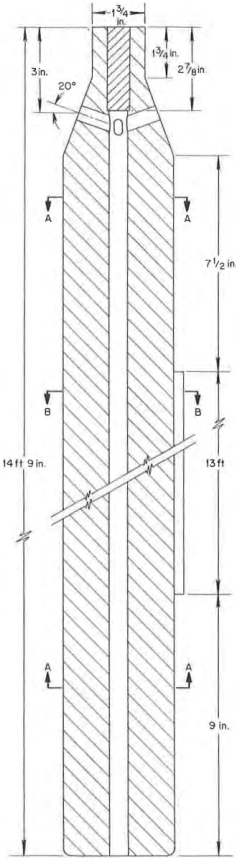
\includegraphics[width=0.25\linewidth]{figs/ch4/zone_i_full_ref.png}
        \label{fig:msbr_i_full_ref}
    }
    \subfloat[][]{
        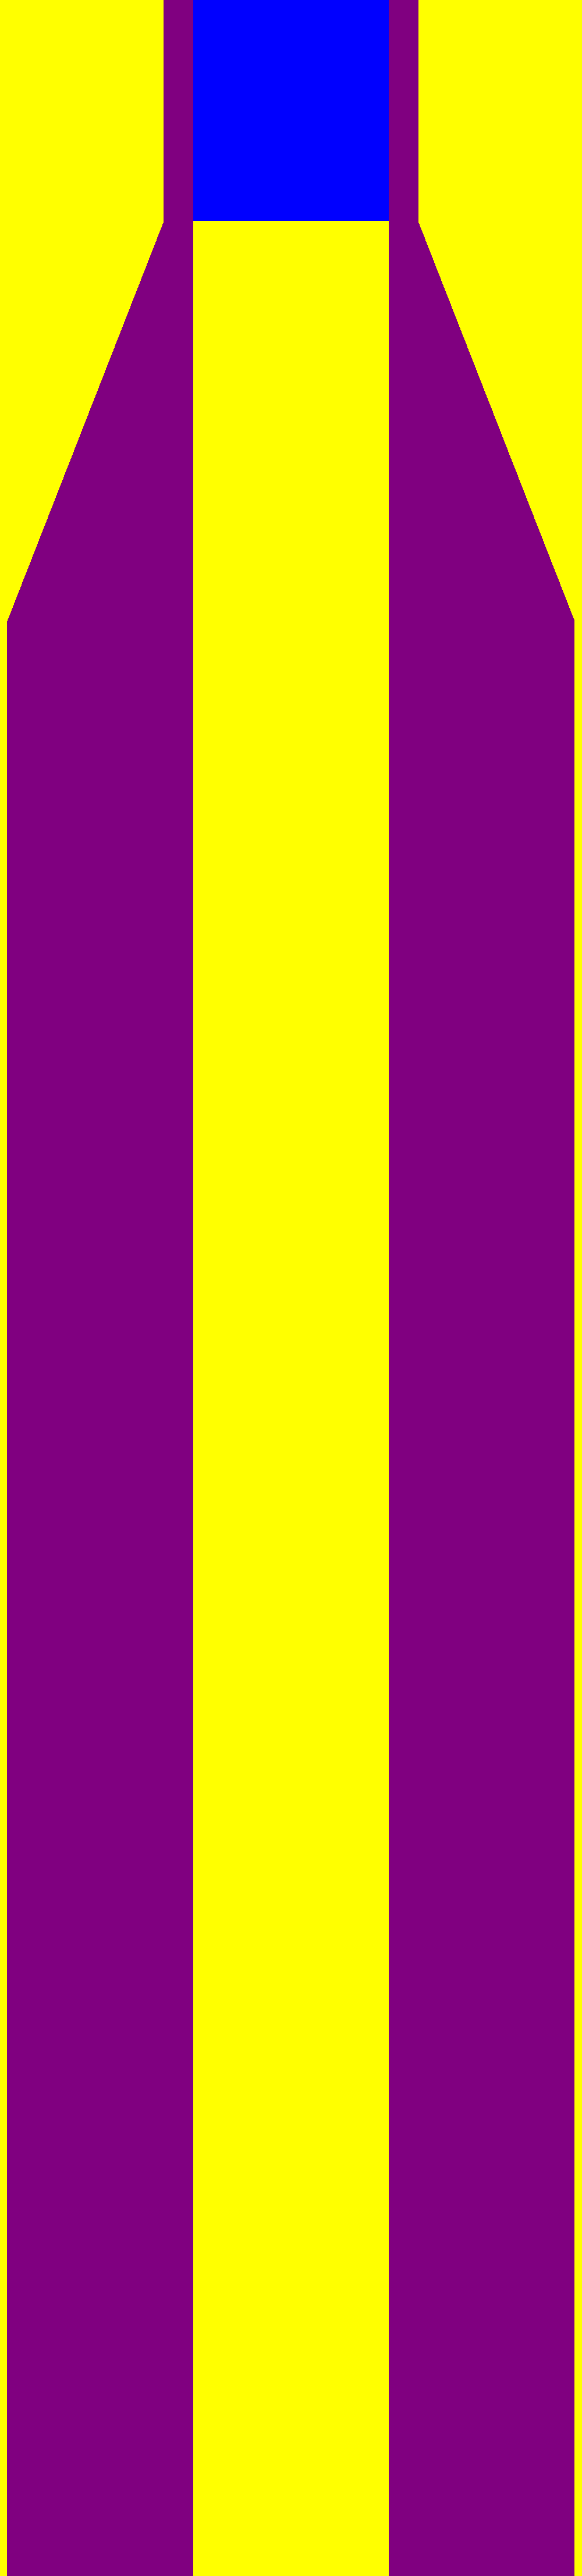
\includegraphics[width=0.17\linewidth]{figs/ch4/zone_ib_full_openmc.png}
        \label{fig:msbr_ib_full_model}
    }
    %\end{tabular}
    \caption[$xz$ cross sections of Zone I elements]{
        \subref{fig:msbr_i_full_ref} Reference Zone I element
        \subref{fig:msbr_ib_full_model} Model Zone I-B element
    }
    \label{fig:msbr-i-xz-full}
\end{figure}

\begin{figure}[htpb]
    \centering
    \subfloat[][]{
        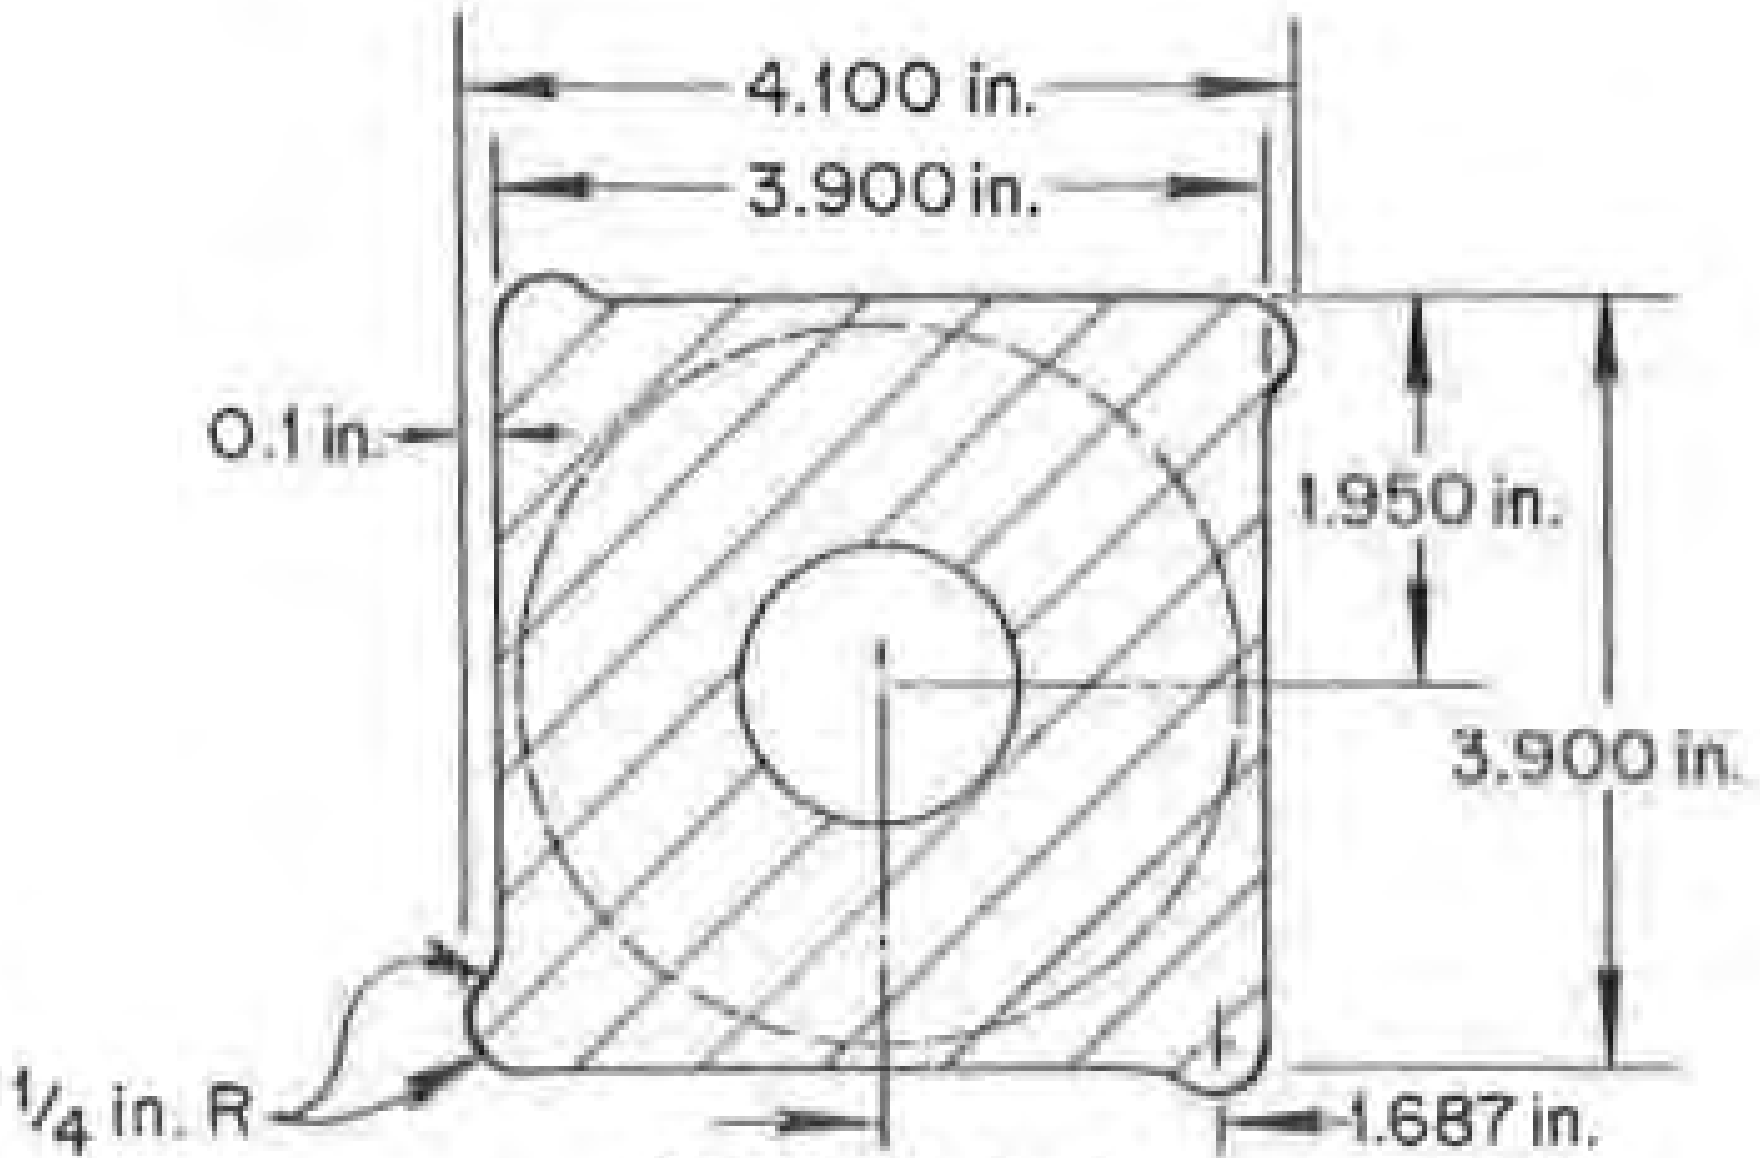
\includegraphics[width=0.3\linewidth]{figs/ch4/zone_ib_main_ref.png}
        \label{fig:msbr_ib_main_ref}
    }
    \subfloat[][]{
        
\includegraphics[width=0.2\linewidth]{figs/ch4/zone_ib_main_openmc.png}
        \label{fig:msbr_ib_main_model}
    }
    \\
    \subfloat[][]{
        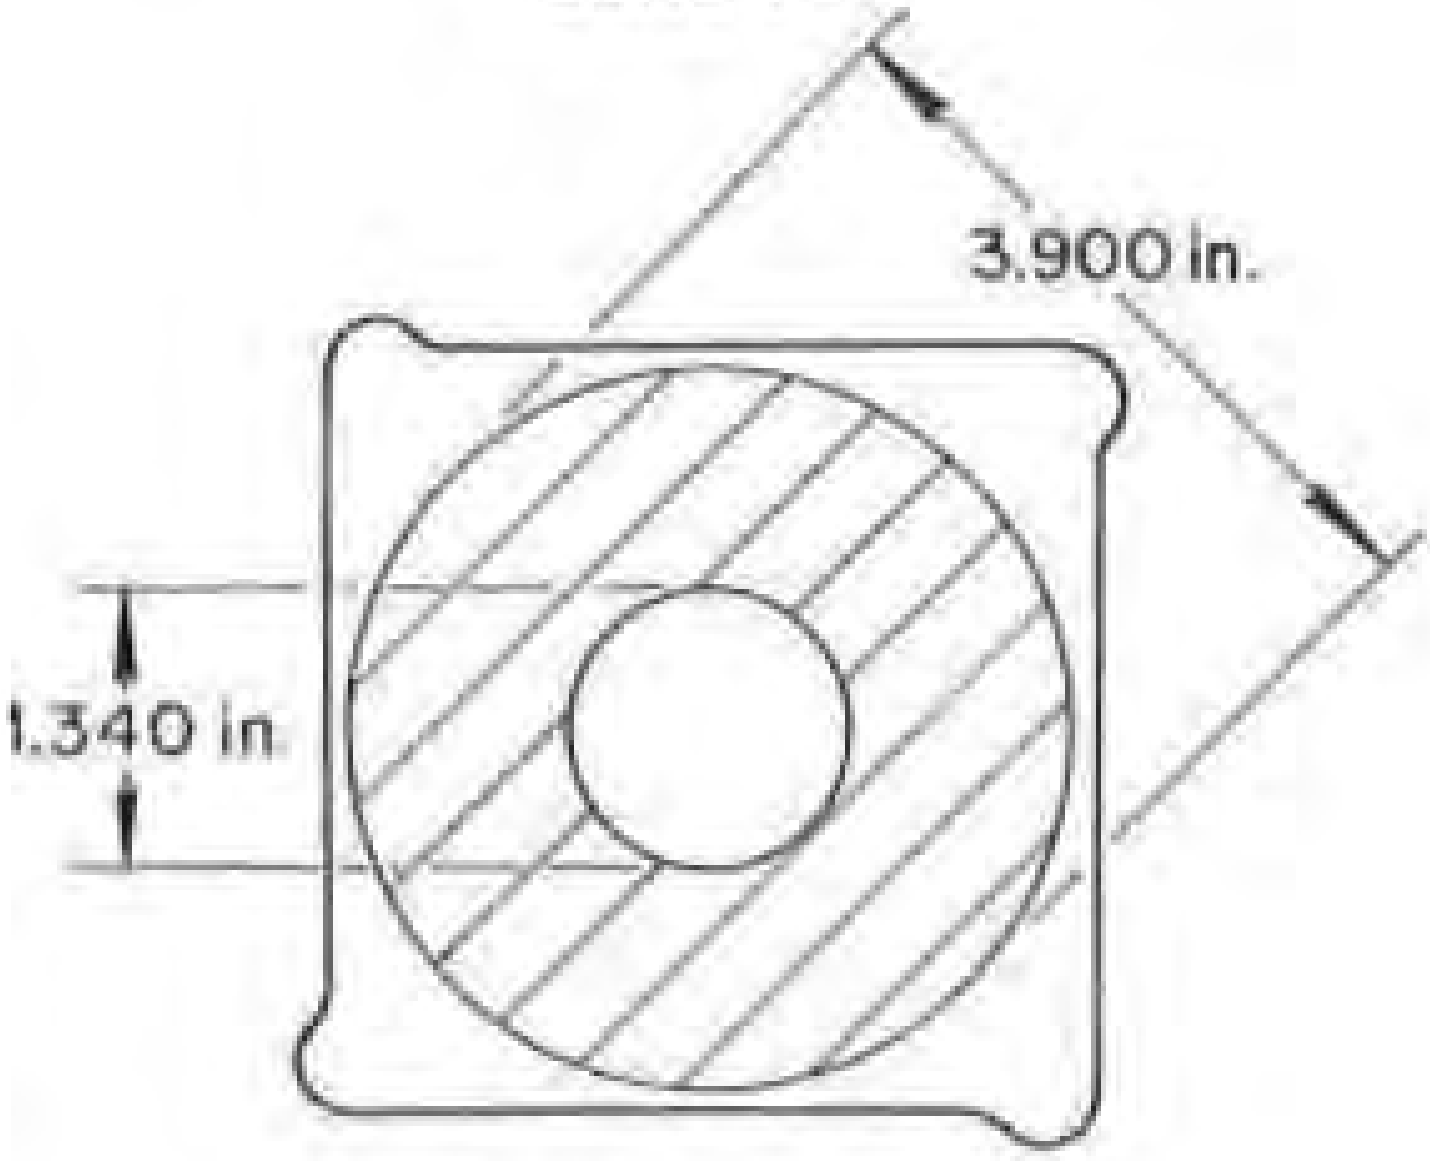
\includegraphics[width=0.3\linewidth]{figs/ch4/zone_ib_bottom_ref.png}
        \label{fig:msbr_ib_bottom_ref}
    }
    \subfloat[][]{
        
\includegraphics[width=0.2\linewidth]{figs/ch4/zone_ib_bottom_openmc.png}
        \label{fig:msbr_ib_bottom_model}
    }
    \caption[$xy$ cross sections of Zone I-B elements]{
        \subref{fig:msbr_ib_main_ref} Reference Zone I-B element; Section B.
        \subref{fig:msbr_ib_main_model} Model Zone I-B element; Section B.
        \subref{fig:msbr_ib_bottom_ref} Reference Zone I-B element; Section A.
        \subref{fig:msbr_ib_bottom_model} Model Zone I-B element; Section A.
    }
    \label{fig:msbr-ib-xy}
\end{figure}

\begin{figure}[htpb]
    \centering
    \subfloat[][]{
        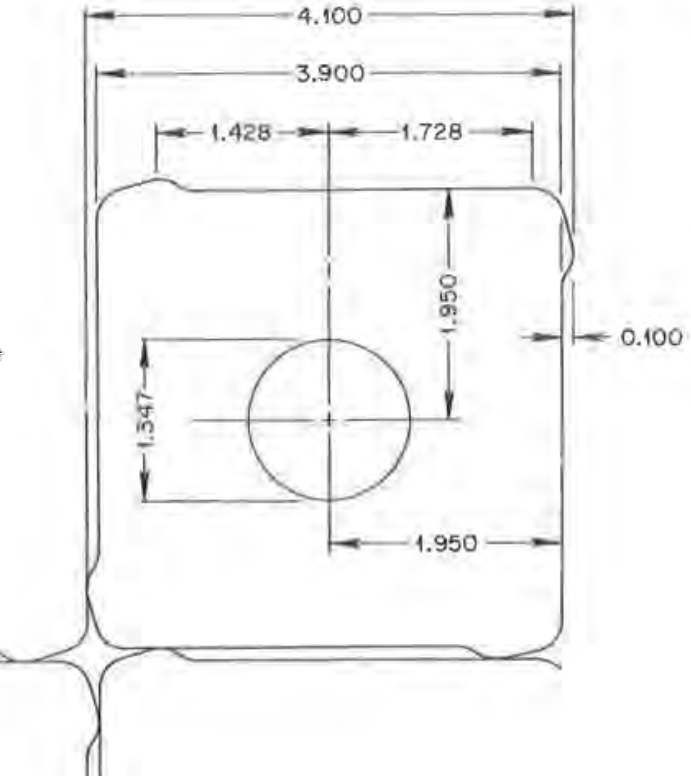
\includegraphics[width=0.25\linewidth]{figs/ch4/zone_ib_lattice_ref.png}
        \label{fig:msbr_ib_lattice_ref}
    }
    \subfloat[][]{
        
\includegraphics[width=0.17\linewidth]{figs/ch4/zone_ib_lattice_openmc.png}
        \label{fig:msbr_ib_lattice_model}
    }
    %\end{tabular}
    \caption[Lattice view of Zone I-B elements]{
        \subref{fig:msbr_ib_lattice_ref} Reference Zone I-B lattice
        \subref{fig:msbr_ib_lattice_model} Model Zone I-B lattice 
    }
    \label{fig:msbr-ib-lattice}
\end{figure}


\begin{figure}[htpb]
    \centering
    \subfloat[][]{
        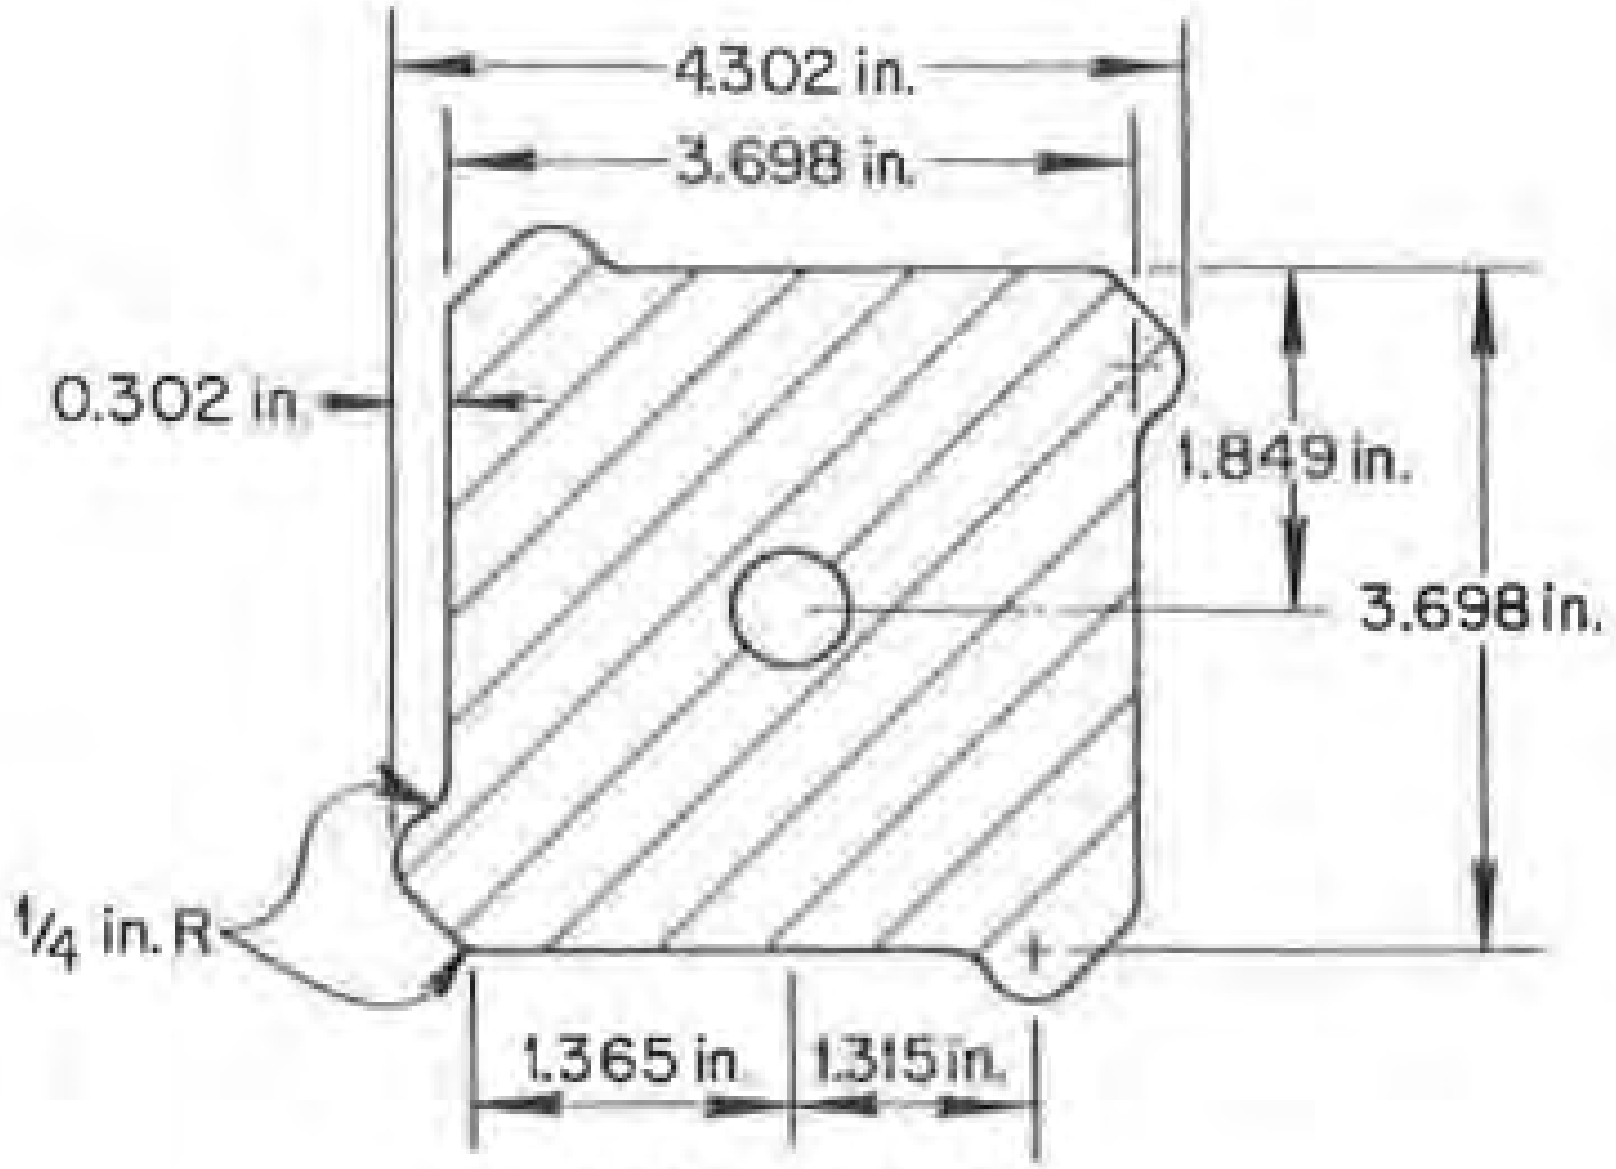
\includegraphics[width=0.3\linewidth]{figs/ch4/zone_ia_main_ref.png}
        \label{fig:msbr_ia_main_ref}
    }
    \subfloat[][]{
        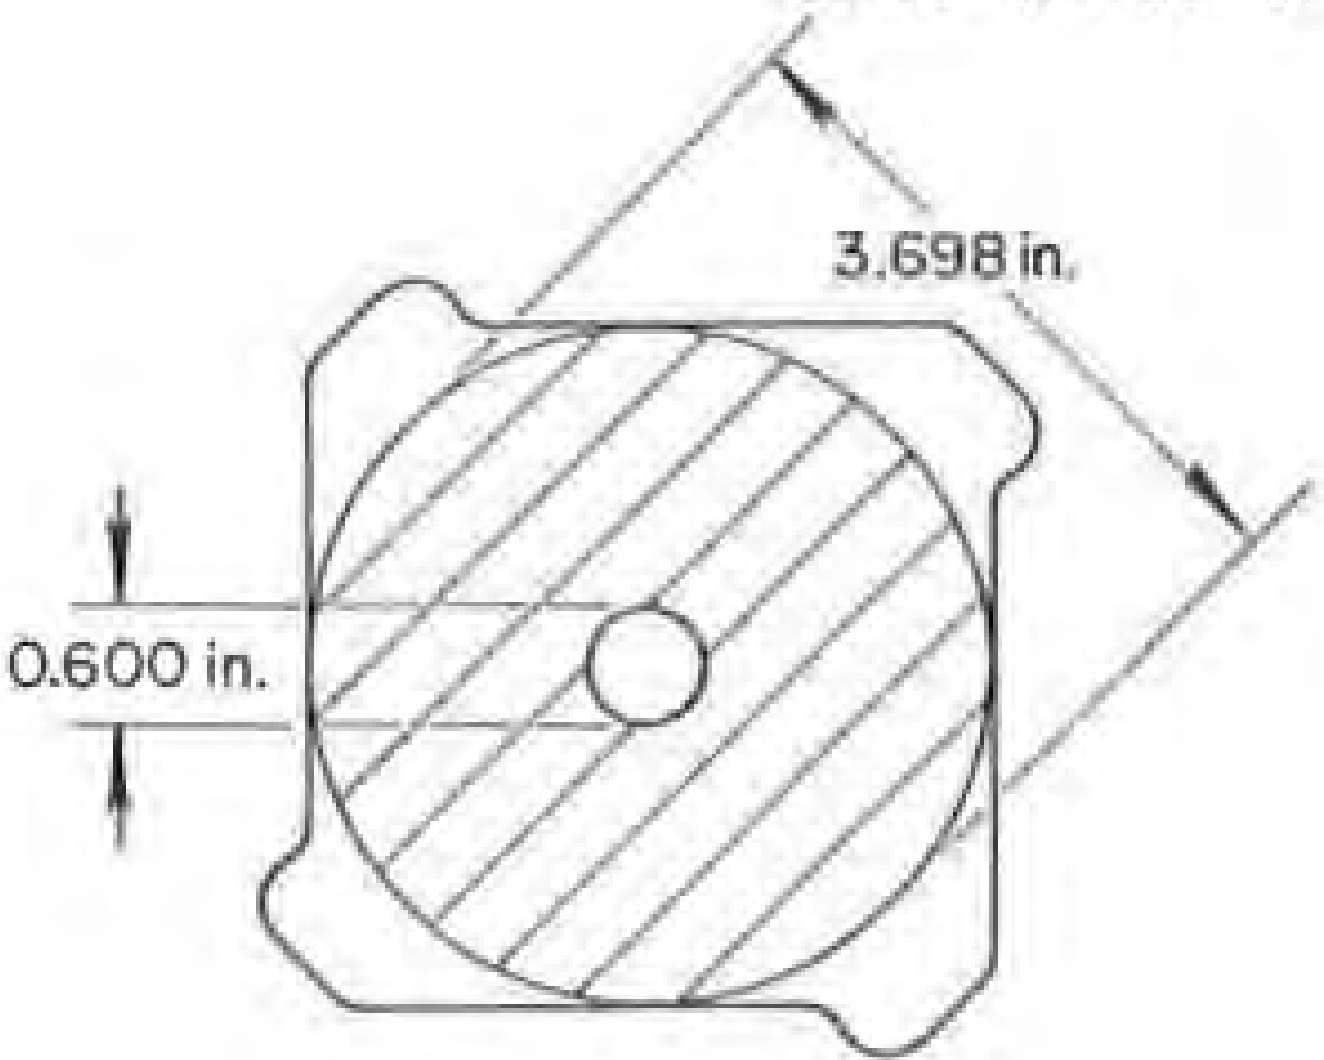
\includegraphics[width=0.3\linewidth]{figs/ch4/zone_ia_bottom_ref.png}
        \label{fig:msbr_ia_bottom_ref}
    }
    \caption[$xy$ cross sections of Zone I-A elements]{
        \subref{fig:msbr_ia_main_ref} Reference Zone I-A element; Section B.
        \subref{fig:msbr_ia_bottom_ref} Reference Zone I-A element; Section A.
    }
    \label{fig:msbr-ia-xy}
\end{figure}

\begin{figure}[htpb]
    \centering
    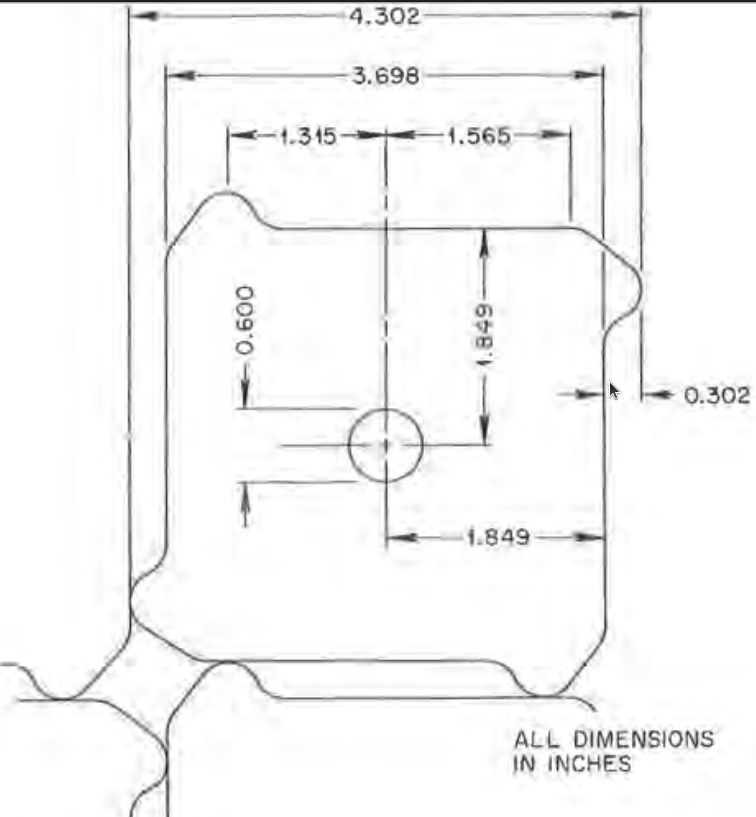
\includegraphics[width=0.25\linewidth]{figs/ch4/zone_ia_lattice_ref.png}
    \caption{Lattice view of Zone I-A elements}
    \label{fig:msbr-ia-lattice}
\end{figure}

Four 6 in.$\times$6 in.
(15.24\unit{\centi\metre}$\times$15.24\unit{\centi\metre}) graphite elements
sit at the center of the core. Two of these elements contain graphite control
rods, and the other two elements are for neutron-absorbing rods for shutting
down the reactor, and are left empty during operation
\cite{robertson_conceptual_1971}. Robertson el al does not specify a design nor
dimensions for the control rod graphite elements. The \Gls{csg} model assumes
that theese elements will be similar in shape to the zone I-A element (see Table
\ref{tab:cr-specification} and Figure \ref{fig:control-rods}). The control rods
themselves have axial passages through them to faciliatate salt flow, but the
dimesions of these passages are not given, so the \Gls{csg} model does not
include them.

\begin{table}[htpb]
    \centering
    \caption{Control rod specifications}
    \label{tab:cr-specification}
    \begin{tabulary}{\linewidth}{|C|CC|CC|}
        \hline
        Quantity & Reference Dimension [in] & Reference Dimension [\unit{\centi\metre}] & Model Dimension [in] & Model Dimension [\unit{\centi\metre}]\\
        \hline
        Control rod element side length & 6 & 15.24 & 5.698 & 14.47292 \\
        \hline
        Control rod element inner diameter & 4 & 10.16 & 4 & 10.16\\
        \hline
        Control rod diameter & 3.75 & 9.525 & 3.75 & 9.525 \\
        \hline
        Rib tip radius of curvature & -  & - & 0.3897638 & 0.99\\
        \hline
        Rib tip to element spacing & - & - & 0.302 & 0.76708 \\
        \hline
        Rib tip to element center & - & - & 3.151 & 8.00354\\
        \hline
    \end{tabulary}
\end{table}

\begin{figure}[htpb]
    \centering
    
\includegraphics[width=0.5\textwidth]{figs/ch4/cr_xy_openmc.png}
    \caption{CSG model control rod lattice}
    \label{fig:control-rods}
\end{figure}


\subsection{Zone II}

Zone II is the undermoderated zone surrounding zone I, and is 37\% fuel salt by
volume. Zone II acts as a blanket zone that reduces neutron leakage from the
core\cite{robertson_conceptual_1971}. Zone II is divided into two subzones: zone
II-A and zone II-B.

Zone II-A consists of elements that are identical to zone I-B elements except
that their cylindrical fuel channel is larger, there is no machining on the bottom part of the elements, and the machining on the top part of the elements is different. (see Table \ref{tab:zone-iia-specs} and Figures \ref{fig:msbr-iia-xz-full} and \ref{fig:msbr-iia-xy}). Half-square triangular graphite elements of the same dimension as the zone II-A elements are present at lattice cells where there would be a nothing connecting zone II-A elements (see Figure \ref{fig:msbr-detail}). 

Zone II-B consists of two different types of elements arranged radially around the core: eight 6 in. (15.24 \unit{\centi\metre}) wide 13 ft. (396.24 \unit{\centi\metre}) tall rectangular slats with holes to fit the 2.5 in. diameter core lifting rods\footnote{the diameter of these holes is unknown, so the \Gls{csg} model assumes they are 6.176 cm in diameter} arranged at 45\unit{\degree} intervals, and 200 (25 between each of the previous type of elements) 2 in. (5.08 \unit{\centi\metre}) wide 13 ft. (396.24 \unit{\centi\metre})
tall rectangular slats of varying length such that the core cross section is
changed from octagonal to circular at the outer bound of zone
II\cite{robertson_conceptual_1971}. These slats have an average length of 10.5
in. (26.67 \unit{\centi\metre}).

The slats have two additional features: dowel pins at the inner periphery that
separate the slabs to create flow passages, and elliptical graphite pins at the
outer periphery that isolates the salt flowing through the core region from the
salt flowing through the reflector region. The slats have axial grooves 1.5 in.
from the outer edge that accomodate the eliptical pins. Robertson et al. does
not specify the precise dimensions or positions  of these pins, so they are not
included in the \Gls{csg} model (see Figure \ref{fig:msbr-detail}).

In addition to the aformentioned simplifications, Figure \ref{fig:msbr-detial}
shows that the \Gls{csg} model makes some notable approximations and
simplifications to the geometry of the individual zone II-B elements which
results in a significantly different appearance than the reference design. Table
\ref{tab:zone-iib-diff} lists these differences.

\begin{table}[htpb]
    \centering
    \caption{caption}
    \label{tab:zone-iib-diff}
    \begin{tabulary}{\linewidth}{|C|C|C|C|}
        \hline
        & 2-in. slats shape & 6-in. slat shape & Pins\\
        \hline
        Reference model & Rectangular prisms ending in a half cylinder & Rectangular prism with deep grooves creating a mixed-concavity surface & Eliptical sealing pins and separating dowel pins\\
        \hline
        \Gls{csg} model & Cylinder sector approximating a rectangular prism & Cylinder sector approximating a rectangular prism & No pins\\
        \hline
    \end{tabulary}
\end{table}

\begin{table}[htpb]
    \centering
    \caption{Zone II-A dimensions}
    \label{tab:zone-iia-specs}
    \begin{tabulary}{\linewidth}{|C|CC|CC|}
    \hline
    Quantity & Reference Dimension [in] & Reference Dimension [\unit{\centi\metre}] & Model Dimension [in] & Model Dimension [\unit{\centi\metre}]\\
    \hline
    Section A inner diameter & 0.5 & 1.27 & 0.5 & 1.27 \\
    \hline
    Section A Outer diameter & 2.875 & 7.3025 & 2.875 & 7.3025 \\
    \hline
    Section B inner diameter & 2.6 & 6.604 & 2.6 & 6.604 \\
    \hline
    Rib tip radius of curvature & 0.25 & 0.635 & 0.263 & 0.66802\\
    \hline
    Rib tip to element spacing & 0.1 & 0.254 & 0.1 & 0.254\\
    \hline
    Rib tip to element center & 1.687 & 4.28498 & 1.687 & 4.28498\\
    \hline
    Section B height & 172 & 436.88 & 172 & 436.88\\
    \hline
    Section A height & 2 & 5.08 & 2 & 5.08 \\
    \hline
    Cone height & 1 & 2.54 & 1 & 2.54 \\
    \hline
    Top part height & 3 & 7.62 & 3 & 7.62 \\
    \hline
    Top part outer radius & 1.75 & 4.445 & 1.75 & 4.445 \\
    \hline
    \end{tabulary}
\end{table}

\begin{figure}[htpb]
    \centering
    \subfloat[][]{
        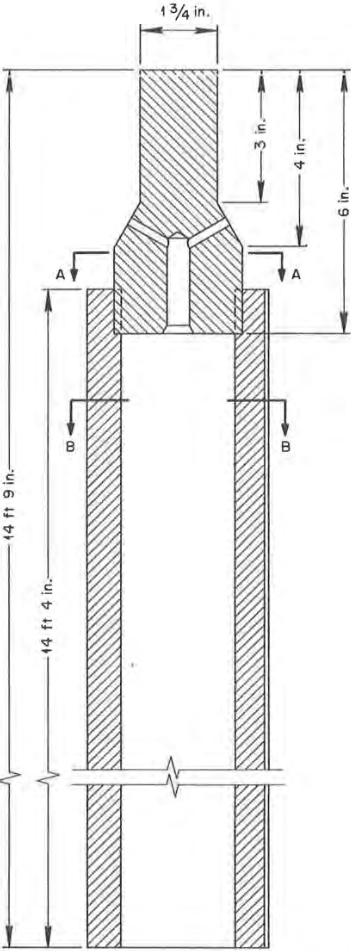
\includegraphics[width=0.25\linewidth]{figs/ch4/zone_iia_full_ref.png}
        \label{fig:msbr_iia_full_ref}
    }
    \subfloat[][]{
        
\includegraphics[width=0.17\linewidth]{figs/ch4/zone_iia_full_openmc.png}
        \label{fig:msbr_iia_full_model}
    }
    %\end{tabular}
    \caption[$xz$ cross sections of Zone II-A elements]{
        \subref{fig:msbr_iia_full_ref} Reference Zone II-A element
        \subref{fig:msbr_iia_full_model} Model Zone II-A element
    }
    \label{fig:msbr-iia-xz-full}
\end{figure}

\begin{figure}[htpb]
    \centering
    %\begin{tabular}{cc}
    \subfloat[][]{
        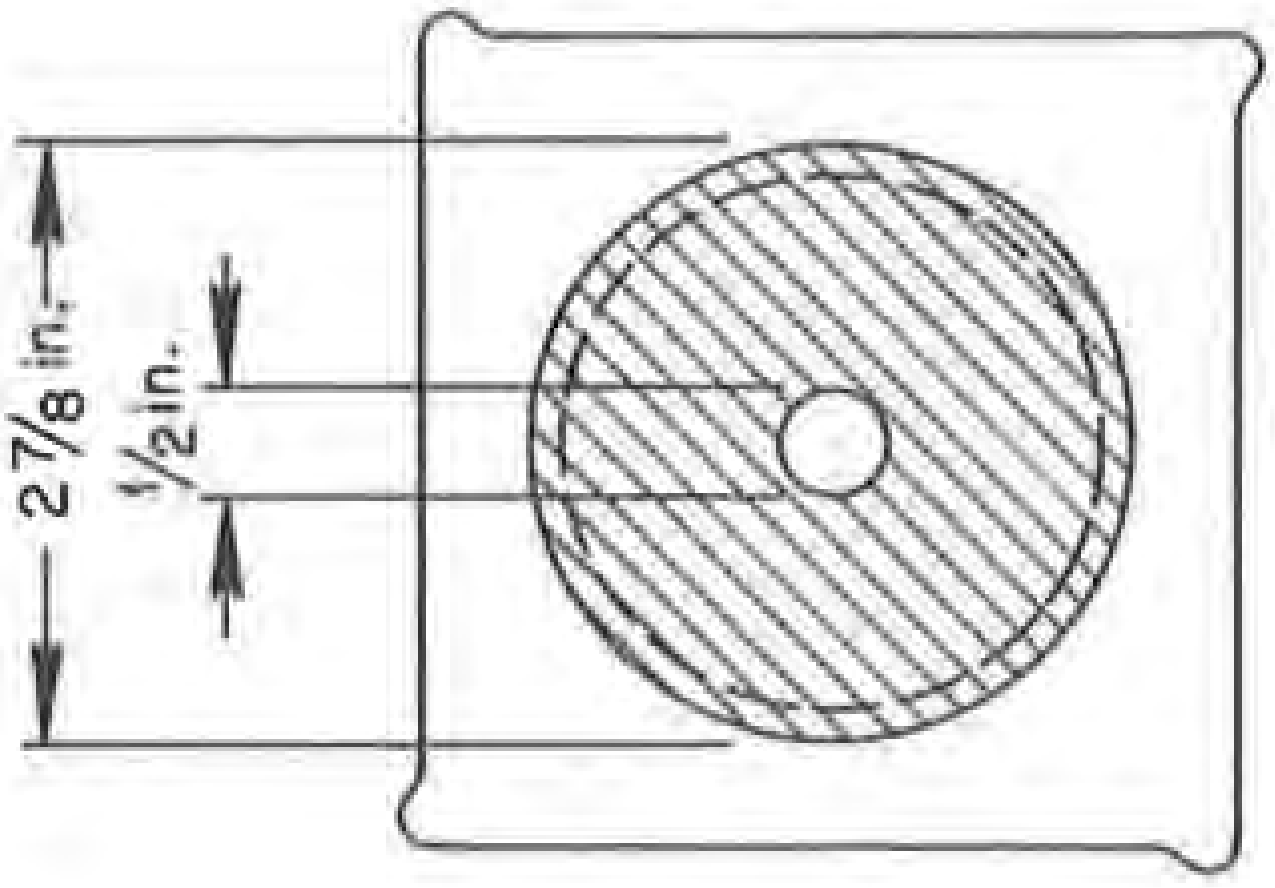
\includegraphics[width=0.3\linewidth]{figs/ch4/zone_iia_top_xy_ref.png}
        \label{fig:msbr_iia_top_ref}
    } 
    \subfloat[][]{
        
\includegraphics[width=0.2\linewidth]{figs/ch4/zone_iia_top_xy2_openmc.png}
        \label{fig:msbr_iia_top_model}
    }
    \\
    \subfloat[][]{
        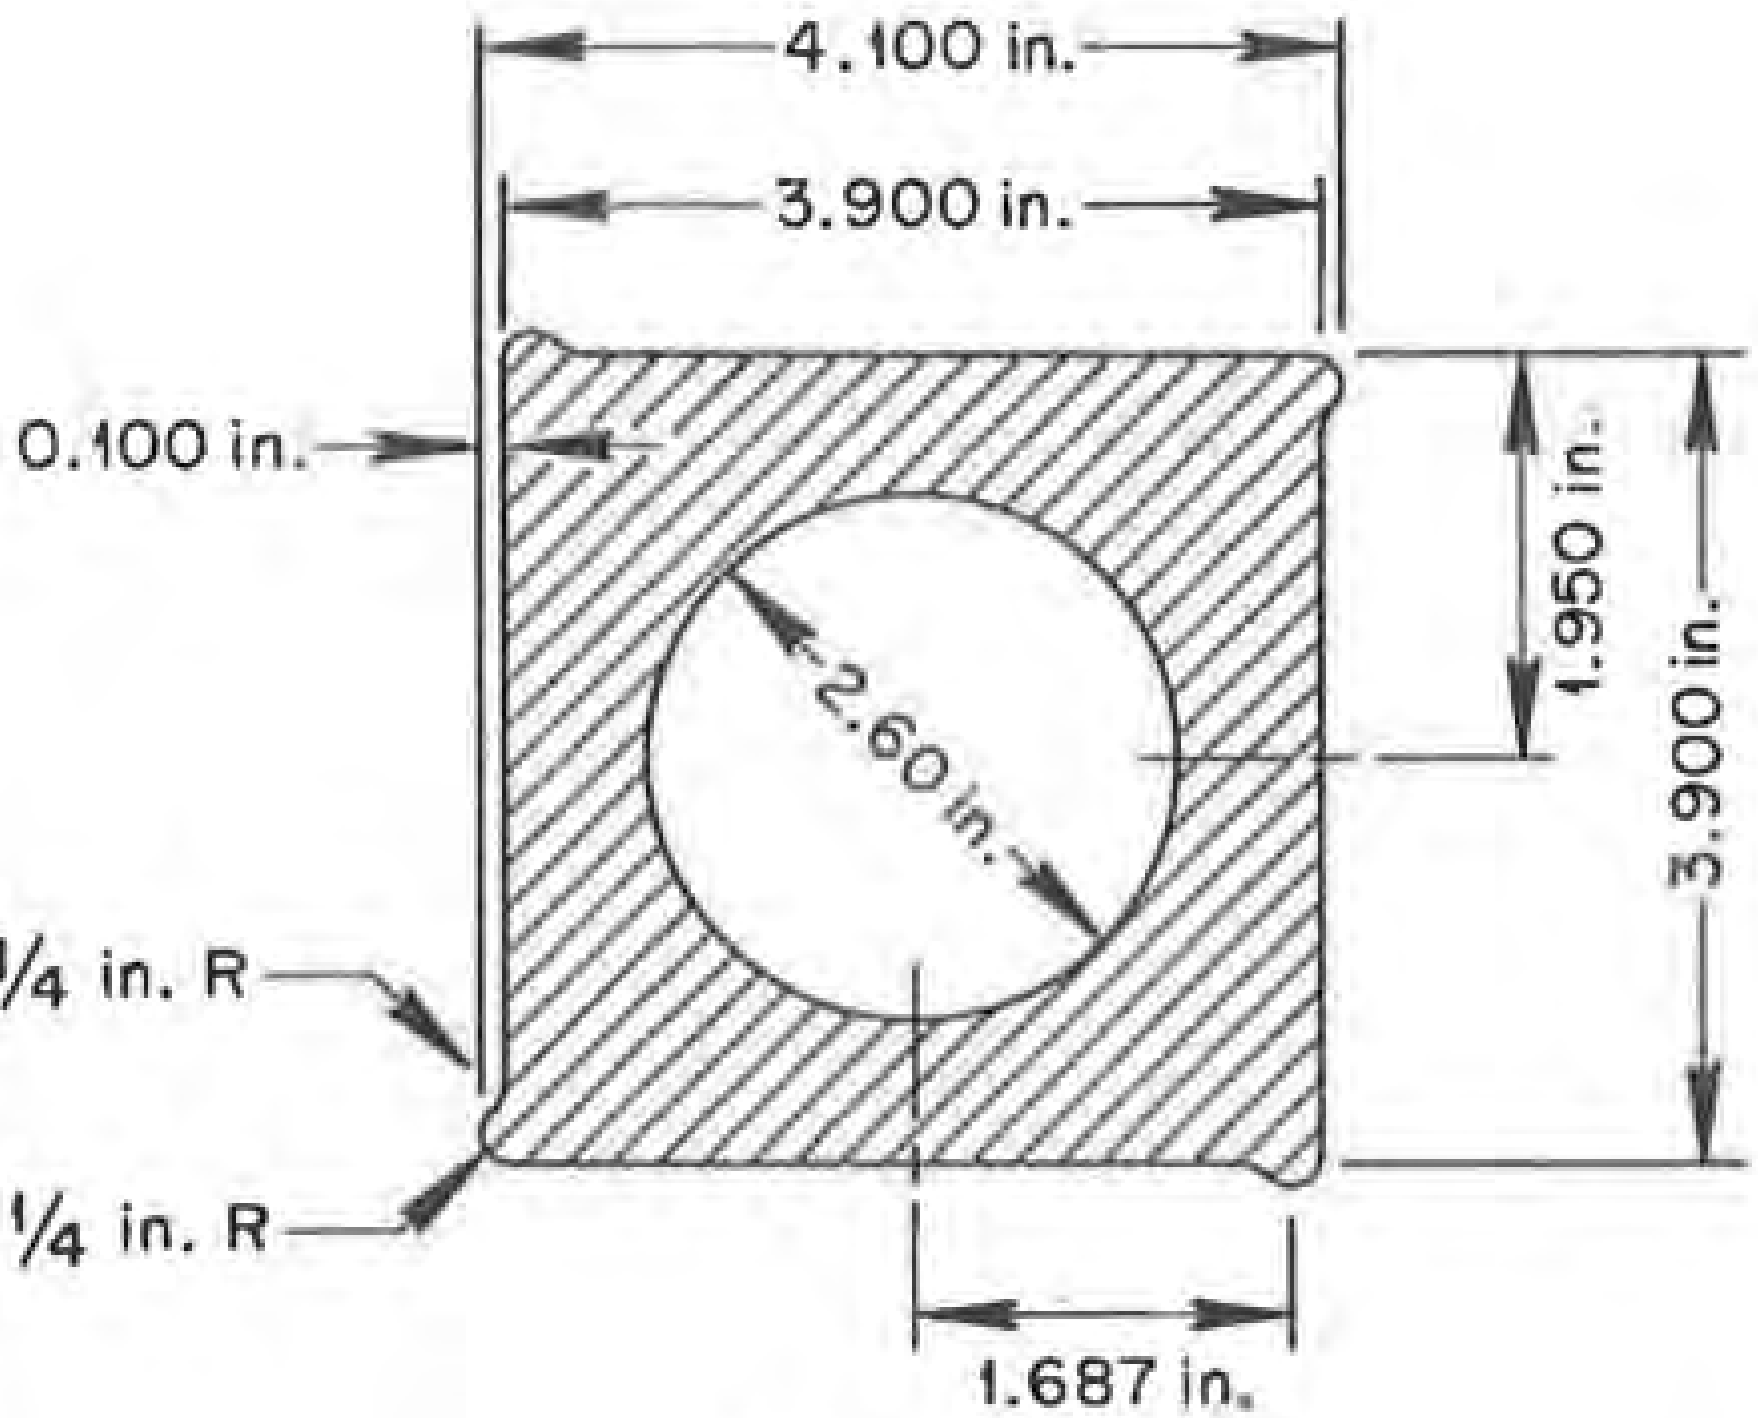
\includegraphics[width=0.35\linewidth]{figs/ch4/zone_iia_main_ref.png}
        \label{fig:msbr_iia_main_ref}
    } 
    \subfloat[][]{
        
\includegraphics[width=0.15\linewidth]{figs/ch4/zone_iia_main_openmc.png}
        \label{fig:msbr_iia_main_model}
    }
    %\end{tabular}
    \caption[$xy$ cross sections of Zone II-A elements]{
        \subref{fig:msbr_iia_top_ref} Reference Zone II-A element; Section A.
        \subref{fig:msbr_iia_top_model} Model Zone II-A element; Section A.
        \subref{fig:msbr_iia_main_ref} Reference Zone II-A element; Section B.
        \subref{fig:msbr_iia_main_model} Model Zone II-A element; Section B.
    }
    \label{fig:msbr-iia-xy}
\end{figure}

\subsection{Annulus}
A 2 in. wide annular space of 100-\% fuel salt separates zone II from the
graphite reflectors. The annulus serves as a clearance space when inserting or
removing the reactor core assembly, and provides some additional shielding to
extend the lifetime of the graphite reflectors\cite{robertson_conceptual_1971}. The annulus region is reproduced in full in the \Gls{csg} model. The annulus region is the dark teal section in between the brown and pink sections in Figure \ref{fig:msbr-cells}

\subsection{Reflectors}
\begin{figure}[htpb]
    \centering
    \subfloat[][]{
        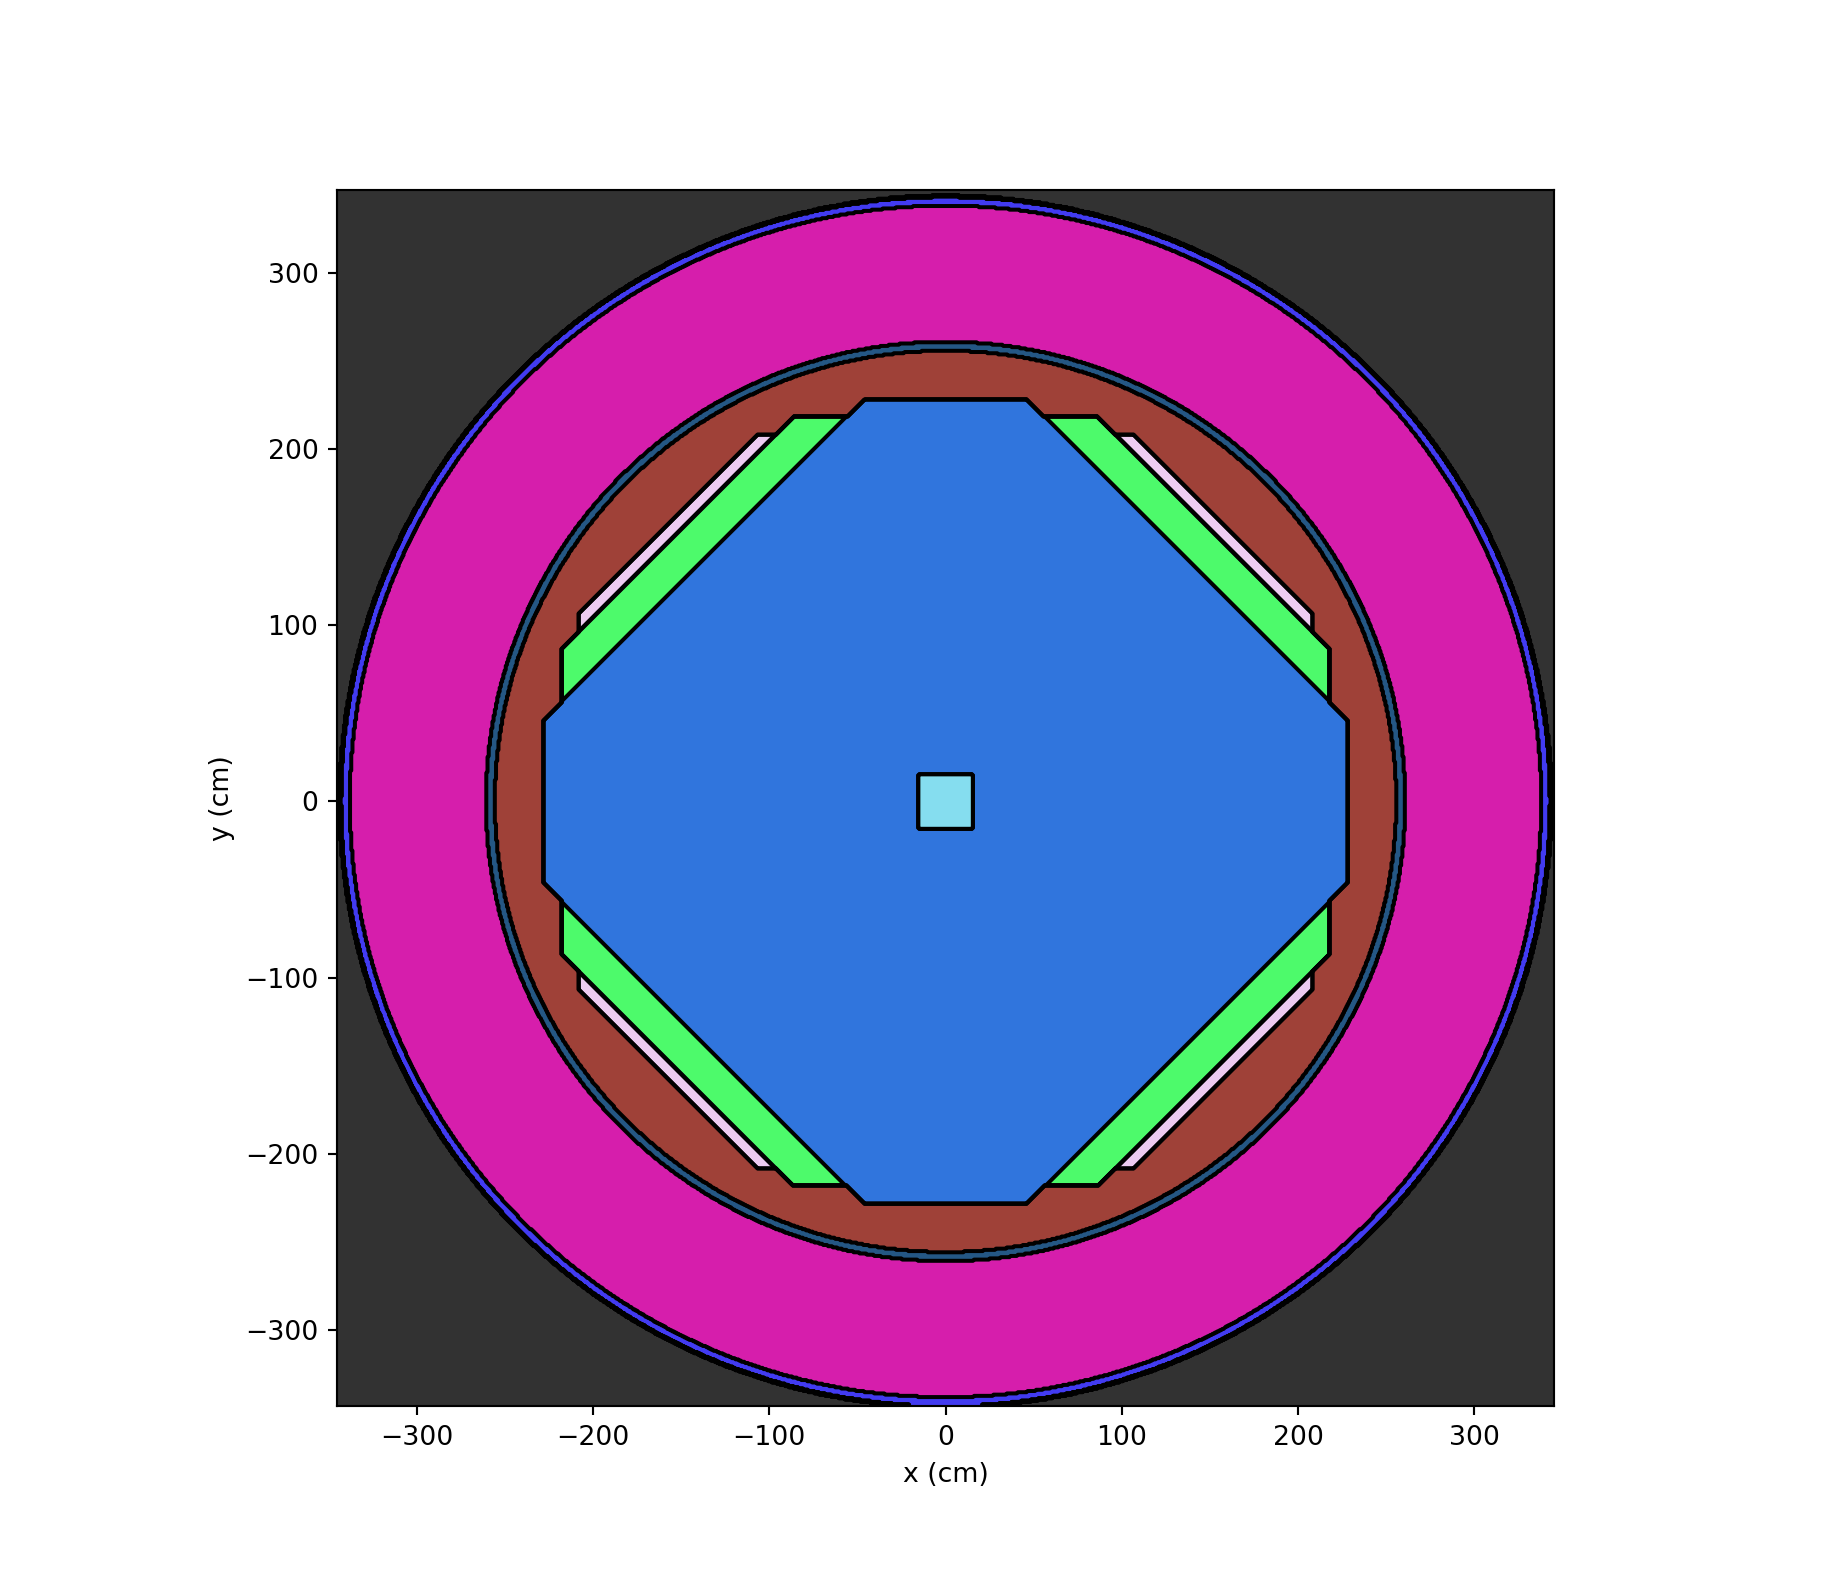
\includegraphics[width=0.5\linewidth]{figs/ch4/msbr_reduced_univs_xy.png}
        \label{fig:msbr-cell-xy}
    }
    \subfloat[][]{
        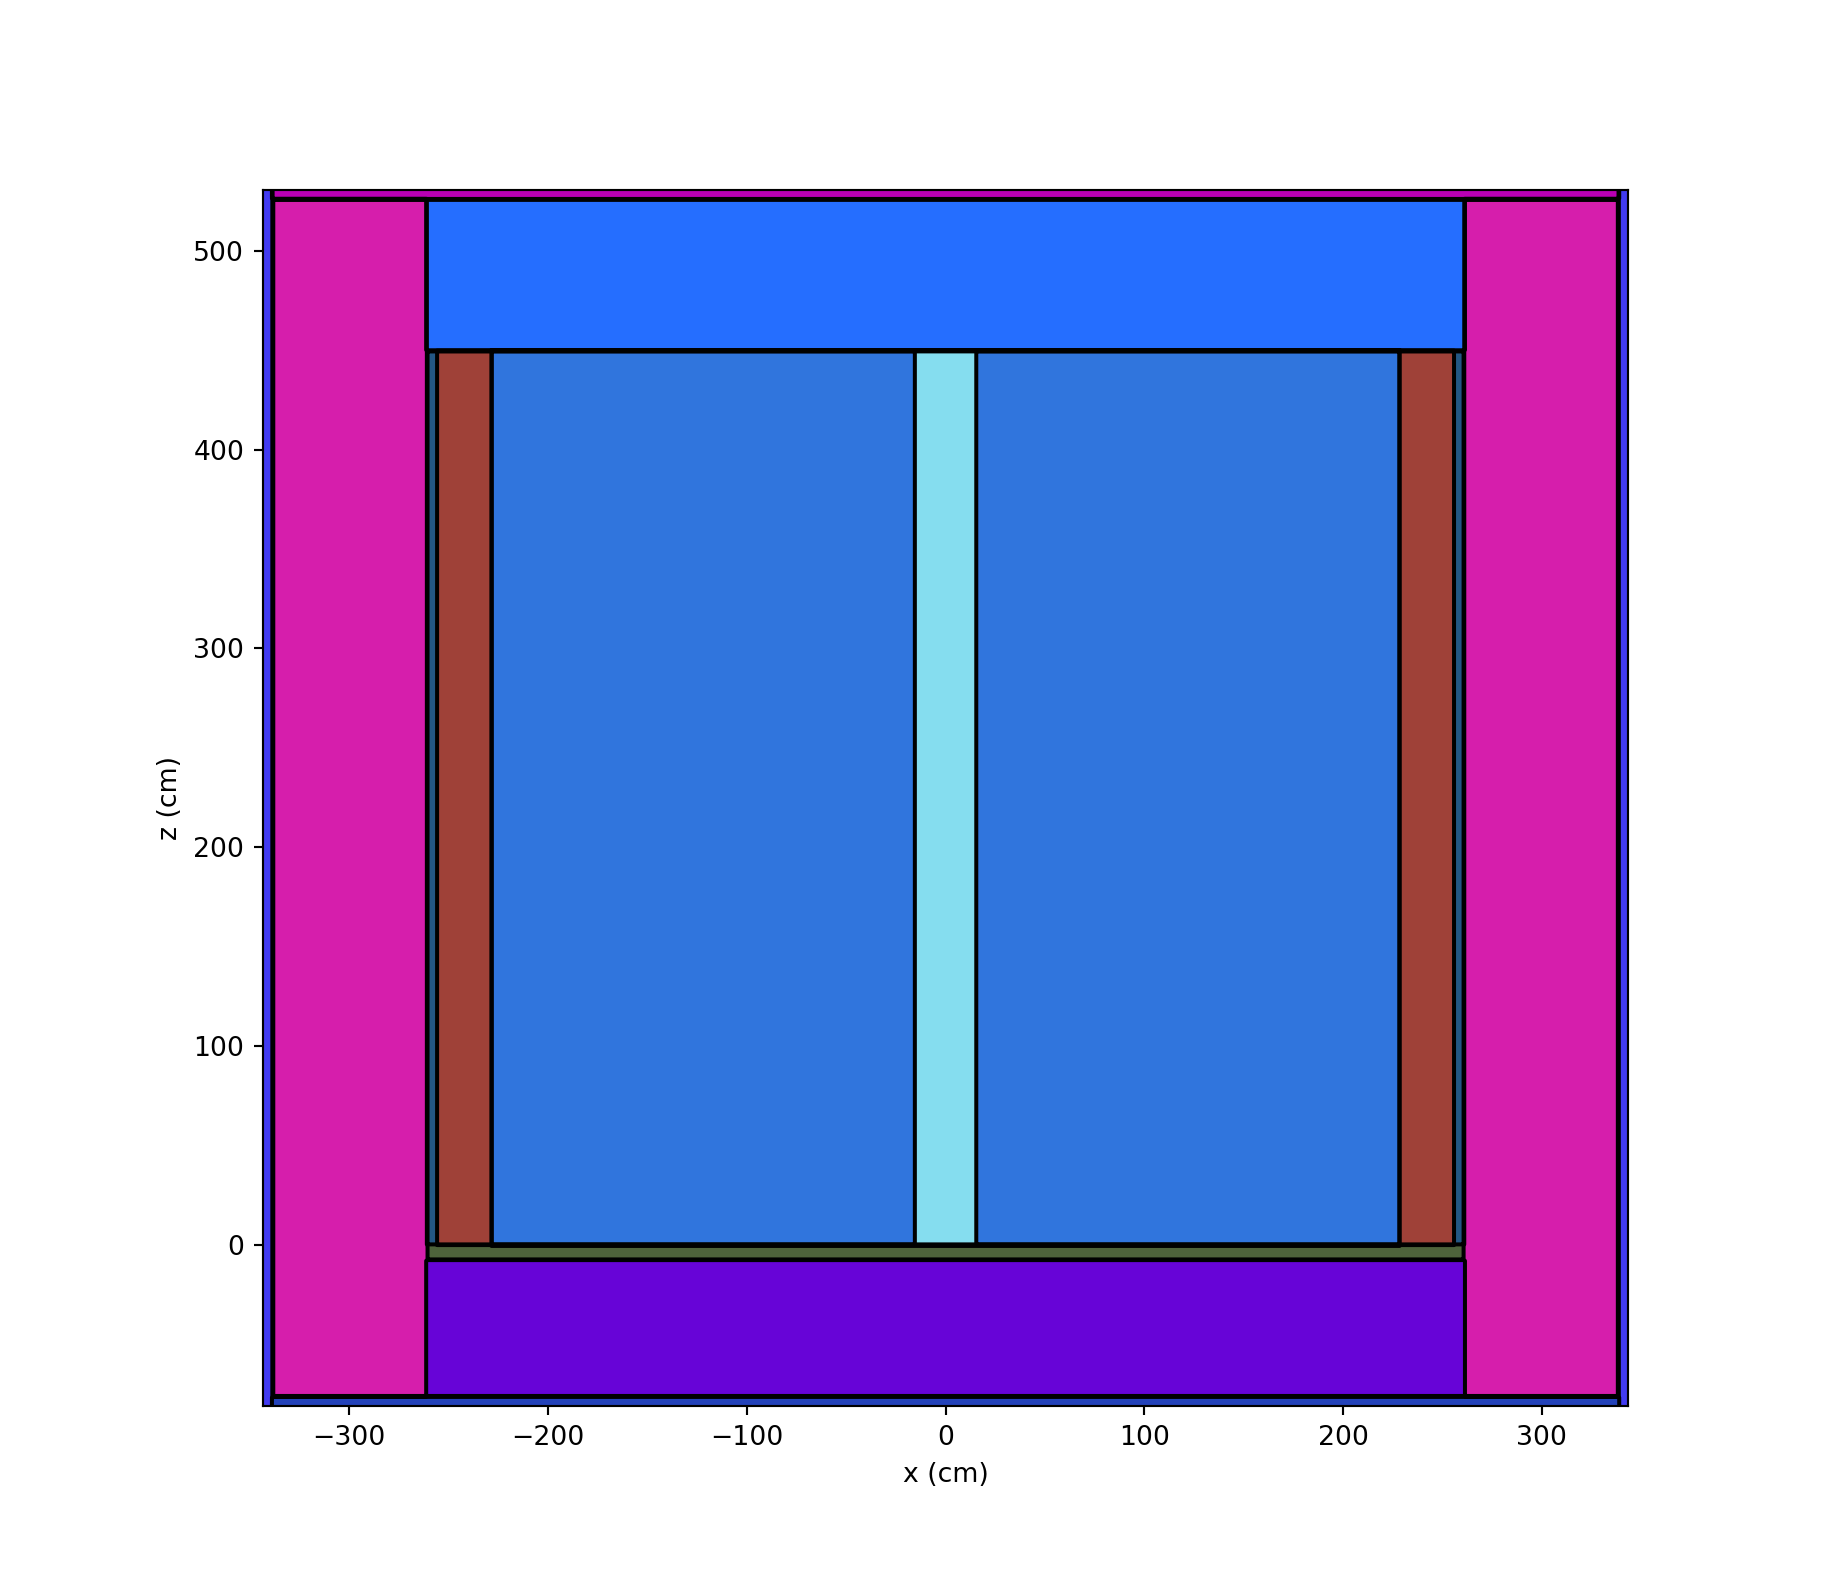
\includegraphics[width=0.5\linewidth]{figs/ch4/msbr_reduced_univs_xz.png}
        \label{fig:msbr-cell-xz}
    }
    \caption[MSBR CSG model cells]{MSBR CSG model cells.
        \subref{fig:msbr-cell-xy} $xy$ plane; 
        \subref{fig:msbr-cell-xz} $xz$ plane} 
    \label{fig:msbr-cells}
\end{figure}
The \Gls{msbr} has both axial and radial reflectors as seen in Figures
\ref{fig:msbr-overview} and \ref{fig:msbr-detail}. Both reflector regions are around 1\% fuel salt by volume. The radial
reflectors\footnote{I exclucde the following details about the radial reflector
due to insufficient information in the report to reproduce them in a model:
Hastelloy N orifice plates, milled radial grooves at the bottom of each
reflector block, top layer blocks (see pages 15 and 16 in Robertson et al.)}
consist of 29 in. (48.26 cm) thick wedge-shaped blocks that are 43 in. tall and 10 in. (25.4 cm) wide at the vessel wall and 9 in. wide at the inner end \cite{robertson_conceptual_1973}.
Four layers of these blocks comprise the entire radial reflector. Slots cut out
of the outer edge of the blocks facilitate Hastelloy N axial ribs to create a
0.25 in (0.635 cm) standoff space between the blocks and the vessel wall. Axial
flow from the reactor inlet through this space cools both the outer portion of
the reflector blocks and the vessel wall. Additionally, Robertson et al. states
that 1 in. graphite pins ``are inserted into the reflector pieces to hold them
apart'', but does not specify the position or number of these pins. These pins
create passages\footnote{these passages change dimension from 0.05 in. wide
while cold to 0.1 in. wide while hot \cite{robertson_conceptual_1971}} for
radial salt flow through the radial reflector region towards the annulus,
providing additional cooling. Hastelloy N retaining rings placed in slots
between the block layers (see Figure \ref{fig:msbr-ref-xz}) ensure that the
position of the reflector blocks to the vessel wall stays relatively constant as
the materials expand under the heating of the fuel salt
\cite{robertson_conceptual_1973}.

The axial reflectors consist of wedge shaped graphite pieces (see Figure
\ref{fig:msbr-ref-xy}) that are 2 in. (5.08 cm) wide at the inner end and 16 in.
(40.64 cm) wide at the outer end \cite{robertson_conceptual_1971}. The dished
vessel heads cause the pieces to vary in thickness from 30 in. (76.2 cm) at the
center to 15 in. (38.1 cm) at the outer end (see Figure
\ref{fig:msbr-ref-xz})\cite{robertson_conceptual_1971}. Robertson et al does not
specify a length for the axial reflector pieces. 

The \Gls{csg} model approximates the complicated structure of the radial
reflector blocks as a hollow cylinder 601.98 cm tall and 77.216 cm thick, and
the axial reflector pieces as flat disks\footnote{the \Gls{csg} model doesn not
include the hole out of the top of the core for the control rods, and flattens
the dish-shape as no dimensions are given to accurately reproduce the curvature
of the axial reflector pieces} 68.58 (bottom)/76.12 (top) cm thick and a radius
of 261.112 cm. The \Gls{csg} model also contains no fuel salt in the reflector
regions. Figure \ref{fig:msbr-cells} shows the radial reflector as a large pink
region, the top axial reflector as a light blue region, and the bottom axial
reflector as a purple region.

\section{Vessel}
\label{sec:msbr-vessel}

\section{Reprocessing system}
\label{sec:msbr-reprocessing-system}

\section{Cross Section Data}

\section{Summary}
